\documentclass{article}

% NeurIPS 2026 style file in its non-anonymous workshop mode, camera-ready copy.
% neurips_2026.sty is the official 2026 style file (2026-01-29), reused
% unmodified from an earlier submission in this project.
\PassOptionsToPackage{numbers,compress}{natbib}
\usepackage[sglblindworkshop,final]{neurips_2026}
\workshoptitle{Foundation Models for Temporal Systems}

\usepackage[utf8]{inputenc}
\usepackage[T1]{fontenc}
\usepackage[hidelinks]{hyperref}
\usepackage{url}
\usepackage{graphicx}
\usepackage{booktabs}
\usepackage{amsmath}
\usepackage{enumitem}
\usepackage{microtype}

% The template puts table captions above the tabular, so it zeroes the space above a
% caption inside a table. Our captions sit below, so restore that space.
\makeatletter
\setlength{\abovecaptionskip}{6\p@}
\setlength{\belowcaptionskip}{\z@}
\renewenvironment{table}
  {\setlength{\abovecaptionskip}{6\p@}%
   \setlength{\belowcaptionskip}{\z@}%
   \@float{table}}
  {\end@float}
\makeatother

% Tighter spacing around the floats, so the main text keeps to four pages.
\setlength{\textfloatsep}{4pt plus 1pt minus 2pt}

% Census count for the displayed top-10, from the pinned 2026-09-07 snapshot
% (audit_results.json, reproducibility_census.displayed_top10.replication_code_no = 9).
\newcommand{\censusTopTenNoCode}{9}
\newcommand{\rtMoiraiIdentical}{no}     % did the two settings agree for Moirai?
\newcommand{\rtFlips}{3}                % ordering changes among the 4 models

% Release link: the authors insert the repository address here.
\newcommand{\supplementurl}{\texttt{REPOSITORY-URL-TO-INSERT}}

% Column heads set on several lines.
\newcommand{\hd}[1]{\begin{tabular}[b]{@{}c@{}}#1\end{tabular}}

\title{What a Forecasting Leaderboard Can Establish:\\ Resolution Reporting for Zero-Shot Time-Series Models}

\author{%
  AUTHOR ONE\\
  AFFILIATION ONE\\
  \texttt{EMAIL-ONE}
  \And
  AUTHOR TWO\\
  AFFILIATION TWO\\
  \texttt{EMAIL-TWO}
}

\begin{document}
\maketitle

\begin{abstract}
A foundation model for time series is pretrained once on a corpus of unrelated series and
then asked to forecast series it has never seen, so its evidence must span many domains.
Independent public forecasting datasets are scarce, so
the field has concentrated its comparisons on one board. GIFT-Eval, the public leaderboard
for zero-shot forecasting, scores every entry on 97 dataset configurations drawn from 28
underlying datasets. It displays a strict order over 128 entries and publishes every
per-configuration score. It does not publish how small a difference 28 datasets can detect.
We name that quantity the \emph{resolution} of the board and introduce \textbf{Vernier}, a
report computed from files a board already publishes. Vernier states the resolution, the
entries inseparable from the leader, and whether the displayed order moves when unrelated
parties submit. GIFT-Eval resolves 6.8 rank places against a median gap of 0.91 between
displayed neighbours, so no neighbouring pair in its top ten separates after correction for
multiple comparisons, under either rank rule it publishes. Replaying its history,
third-party submissions reversed 20 pairs of entries that were never rerun. The
pool-independent geometric mean of scaled error reversed none. On four more boards,
rank-based rules reversed such pairs wherever the history could be replayed, and every board
built from 15 to 39 public data sources displays neighbours 3 to 20 times closer than it can detect. One
choice no board records is the history a model is given. Shortening it to 512 steps raises
the error of three of four open models on 70 configurations, Moirai-2.0 by 6.2\% and
TimesFM-2.5 and Toto by 15.3\% each. We release Vernier, the pinned snapshot, and a
disclosure list for temporal evaluation.
\end{abstract}

\section{Introduction}

Foundation models for time series are pretrained on large heterogeneous corpora and then
applied to series that were absent from training. The distinguishing claim is not accuracy
on one dataset but transfer to datasets nobody chose in advance, so the evidence has to
span many domains, sampling frequencies, and horizons. Public forecasting datasets that are
genuinely independent of one another are scarce, and nearly every comparison between these
models now runs through one public board.

That board is GIFT-Eval \citep{gifteval}. It evaluates every submission on the same 97
dataset configurations. A configuration is one dataset at one sampling frequency and one
forecast horizon. The board displays a strict order over 128 entries, and its
per-configuration scores are public. Model releases announce positions on it, and papers
cite a position as evidence of state-of-the-art accuracy \citep{timerouter}.

Every measurement has a resolution, which is the smallest difference it can separate from
noise. Leaderboards report none. The omission matters here, because the evidence base is
narrow and its units are not independent. The 97 configurations come from 28 underlying
datasets, four of which contribute eight configurations apiece, so configurations from one
dataset rise and fall together. An evidence base of that shape cannot support arbitrarily fine
distinctions, and the board displays them to the rank place.

We therefore ask three questions a board can answer about itself without rerunning a single
model, given the per-configuration scores it already publishes. How small a difference can
it detect, which of its displayed distinctions does that permit, and does its order depend
on which other models happen to have been submitted?

\paragraph{Contributions.} \textbf{Vernier} answers those questions from a board's own
files, at no additional compute (\S\ref{sec:vernier}). GIFT-Eval resolves 6.8 rank places
against a median gap of 0.91, and no neighbouring pair in its top ten separates after
correction for multiple comparisons, a pattern that holds on every other board built from 15
to 39 public data sources (\S\ref{sec:boards}). Below the resolution a mean-rank rule assigns part of the order to the
rest of the pool, so third-party submissions reversed 20 pairs of untouched entries, and
none under the pool-independent rule the board also publishes. The history a model receives,
which no board records, raises the error of three of four open models on 70 configurations
(\S\ref{sec:protocol}).

\section{Related work}

\paragraph{Forecasting benchmarks that report uncertainty.} fev-bench reports paired
bootstrap intervals over its tasks \citep{fevbench}, and TS-Arena collects forecasts before
the outcome exists and reports bootstrapped rating intervals \citep{tsarena}. The order this field cites is GIFT-Eval's, and it publishes no
interval of any kind.

\paragraph{How ranks behave under uncertainty.} Rank intervals have been constructed for
language-model and tabular leaderboards \citep{rankint1, rankint2}, and a quantization audit
proposes fixing the detectable difference before running \citep{pairedmde}. That a mean-rank
comparison depends on the remaining pool is established \citep{benavoli2016, zhanghardt2024}
and has been measured on language-model arenas \citep{arenaperturb}. None of it addresses a
forecasting board, whose units are datasets and whose pool is small enough for one submission
to matter.

\paragraph{Evaluation practice for pretrained forecasters.} Recent work revisits evaluation
practice in long-horizon forecasting \citep{positionpaper} and audits pretraining corpora for
contamination against the datasets these boards use \citep{tsfmaudit}. One benchmark sweeps
the history length supplied to a model \citep{tsfmbench}, but none measures how finely the
boards resolve their order.

\section{What Vernier computes}
\label{sec:vernier}

\paragraph{How small a difference can the evidence base detect?} The configurations are a
sample of the domains a pretrained model might meet, so a difference between two entries
carries sampling error. We estimate it with a standard error clustered by dataset, the honest
treatment when eight configurations share one source, using the CR2 small-sample correction
and Satterthwaite's degrees of freedom, 11 to 17 on GIFT-Eval
\citep{bellmccaffrey2002, imbenskolesar2016}. The \textbf{resolution} is the smallest true
difference this design detects eight times in ten at the five percent level, $(t_{0.975} +
t_{0.80})$ standard errors, taken as the median over the nine neighbouring pairs of the
displayed top ten in the units the board displays. CR2 replaces the submitted version's
percentile bootstrap, which declared too many differences (Appendix~\ref{app:calib}).

\paragraph{Which entries cannot be separated from the leader?} For each pair among the
displayed leaders we test their difference with CR2. A gap counts as established when the
test rejects at 5\%, and we give counts before and after the Holm correction
\citep{holm1979}, with the wild cluster bootstrap \citep{cameron2008} and exact sign-flip
tests beside it (Appendix~\ref{app:method}). Entries that never separate from the leader form its \textbf{tier}, the display a
board can defend in place of a strict order.

\paragraph{Does the order depend on who else submitted?} A mean-rank rule scores an entry
against the rest of the pool, so an unrelated submission can move it, and a board's version
history answers whether that happens in practice. We replay the history update by update,
skipping any update in which the evaluation set itself changed. At each update we count the
pairs of entries from the prior displayed top ten whose own result and metadata files are
unchanged and that exchange places. We call this the \textbf{bystander test}.

\section{Results}
\label{sec:boards}

\begin{table}[t]
\centering
\scriptsize
\setlength{\tabcolsep}{2.5pt}
\renewcommand{\arraystretch}{0.9}
\begin{tabular}{@{}llrrrcl@{}}
\toprule
\textbf{Board and rule} & \hd{\textbf{Independent}\\\textbf{sources}} & \textbf{Resolution} & \hd{\textbf{Median gap,}\\\textbf{neighbours}} & \textbf{Ratio} & \hd{\textbf{Neighbours}\\\textbf{separated}} & \hd{\textbf{Untouched top-ten}\\\textbf{pairs reversed}} \\
\midrule
GIFT-Eval, mean rank on MASE$^\dagger$ & 28 datasets & 6.80 & 0.91 & 7.5 & 1 & \textbf{20 in 14 of 141 updates} \\
GIFT-Eval, geometric mean & 28 datasets & 0.0497 & 0.0045 & 11 & 0 & 0 in 141 \\
fev-bench, win rate$^\dagger$ & 39 families & 7.51 & 2.08 & 3.6 & 0 & \textbf{2 in 2 of 30} \\
fev-bench, skill score & 39 families & 3.20 & 0.83 & 3.9 & 0 & 0 in 30 \\
Chronos Benchmark II, mean rank$^\dagger$ & 19 sources & 4.24 & 0.22 & 19 & 0 & \textbf{8 in 3 of 11} \\
Chronos Benchmark II, geometric mean & 19 sources & 9.29 & 0.59 & 16 & 0 & 0 in 11 \\
TIME, geometric mean (displayed) & 39 datasets & 0.0238 & 0.0021 & 11 & 0 & 0 in 44 \\
TIME, MASE rank column$^\dagger$ & 39 datasets & 4.01 & 0.378 & 11 & 1 & \textbf{13 in 12 of 44} \\
BOOM, each series independent$^\dagger$ & 2,554 series & 0.196 & 0.312 & 0.63 & 9 & history too short \\
BOOM, grouped by domain$^\dagger$ & 23 domains & 0.635 & 0.312 & 2.04 & 5 & history too short \\
\bottomrule
\end{tabular}
\caption{Vernier on five boards. A dagger marks a rule that ranks an entry against the others;
ratio is resolution over median gap; neighbours separated are of 9, CR2, uncorrected (units in
Appendix~\ref{app:boards}). GIFT-Eval is pinned on 2026-09-07; the other boards were read in November 2026, TIME with results to 2026-10-31. GIFT-Eval's
20 reversed pairs (exact tie-break) are 18 with ties averaged.}
\label{tab:report}
\end{table}

\paragraph{The board displays distinctions its evidence cannot carry.} No gap between
neighbouring entries in GIFT-Eval's top ten separates after the Holm correction, under CR2,
the wild cluster bootstrap or the exact tests (Appendix~\ref{app:gaps}). Twenty-eight
datasets resolve 6.8 rank places, while the median gap between displayed neighbours is 0.91,
so the board separates entries 7.5 times more finely than its evidence allows.
Widening the evidence to carry those distinctions would take roughly 48 times as many
datasets, which is beyond the near-term supply of independent forecasting series. Beyond the
neighbours, only 12 of the 45 top-ten pairs
separate under CR2, 9 under the earlier rank rule the board still publishes, and none
survives a Holm correction under either (Appendix~\ref{app:counts}). No adjacent
gap on GIFT-Eval or fev-bench reaches its own resolution (Figure~\ref{fig:gaps}). On
fev-bench \citep{fevbench}, Chronos Benchmark II \citep{chronos} and TIME \citep{timebench},
as on every board built from 15 to 39 public data sources, neighbours sit 3 to 20 times closer than the
board can detect, and at most one of nine separates. BOOM \citep{boom} separates all nine if
each of its 2,554 series counts as independent evidence, and five when its series are grouped
by domain (Appendix~\ref{app:boards}).

\begin{figure}[t]
\centering
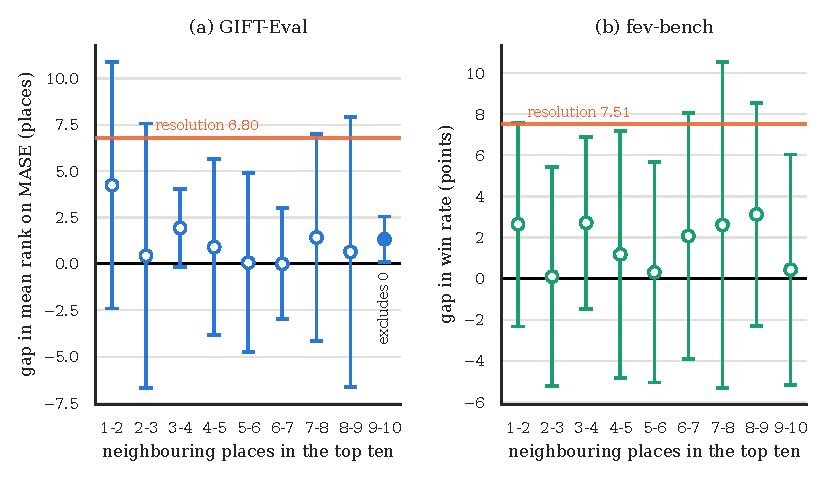
\includegraphics[width=0.68\textwidth,height=0.115\textheight,keepaspectratio]{fig_resolution.pdf}
\caption{Adjacent gaps in the displayed top ten of GIFT-Eval (a) and fev-bench (b), with CR2
95\% intervals, against that board's own resolution.}
\label{fig:gaps}
\end{figure}

\paragraph{Below the resolution the pool decides the order.} A mean-rank rule scores an
entry by ranking it against every other entry on each configuration, so an arrival nobody
reran still displaces the models already on the board. That displacement is small, but it
decides the display wherever the gap is smaller still, which on GIFT-Eval is most of the top
ten. Between 2026-08-31 and 2026-09-07 the board took three submissions
from three unrelated organisations and changed nothing else, and the order of Falcon-Agent,
CastStar and limix\_moe reversed completely (Appendix~\ref{app:perturb}). Twenty such
reversals sit in the board's
history, spread over fourteen updates, nine of them in 2026 (Appendix~\ref{app:replay}). The
geometric mean of scaled error never ranks an entry against the pool, so by construction it
reverses nothing over the identical history. On fev-bench, Chronos Benchmark II and TIME the
rules using only an entry's own scores also reversed nothing, while the rank-based rules
reversed 2, 8 and 13 untouched pairs. The submitted version called fev-bench stable on a
drop-one check, and its history, now available, shows otherwise (Appendix~\ref{app:boards}).

\paragraph{Tiers change what the board recommends.} All ten entries at the top are agentic
pipelines, which select or combine several forecasters per series. Nine of the ten declare no reproduction code
(Appendix~\ref{app:census}). Read as a strict order, the board points a practitioner toward a
system they cannot rebuild. Read as tiers under the pool-independent rule, the leader's tier
holds 17 entries under CR2, and one of them is TimesFM-3, a pretrained model released with
weights \citep{timesfm}. CR2 does not hold its level on this rule, but a signed-rank test on
dataset means does, and its tier of 16 also holds TimesFM-3 (Appendix~\ref{app:tiers}). The
choice between a
routing system and a downloadable checkpoint is not settled by this evidence.

\section{The setting no board records}
\label{sec:protocol}

Resampling published scores cannot expose sensitivity to how an evaluation was configured,
because score files record no configuration. For a pretrained forecaster the choice left
most open is the length of history it receives before forecasting. Pretraining fixes a
maximum context and each release documents a recommended value, but none of this reaches the
board. We evaluated four open models at
two settings each on all 70 configurations whose median series holds at least 1,024 steps,
from 18 datasets in 14 sources, 12 of which the submitted version ran
(Appendix~\ref{app:history}). The models are
Chronos-Bolt-base \citep{chronos}, Moirai-2.0-R-small \citep{moirai}, TimesFM-2.5-200M
\citep{timesfm} and Toto-Open-Base-1.0 \citep{toto}, run inference only. The first setting is
the value in GIFT-Eval's own reference notebook for that model, and the second is a history of
512 steps. The estimate and the tests were fixed before the runs.

\begin{table}[t]
\centering
\scriptsize
\setlength{\tabcolsep}{3pt}
\begin{tabular}{@{}lllll@{}}
\toprule
\textbf{Model} & \hd{\textbf{Change in error at 512 steps,}\\\textbf{70 configurations [95\% interval]}} & \hd{\textbf{$p$ after}\\\textbf{Holm}} & \hd{\textbf{Change on the 58}\\\textbf{outside the twelve}} & \hd{\textbf{Change on the}\\\textbf{first twelve}} \\
\midrule
Chronos-Bolt-base\,$^\dagger$ & +2.7\% [$-$0.9, +6.2] & 0.11 & +3.7\% & $-$2.0\% \\
Moirai-2.0-R-small & \textbf{+6.2\%} [+1.6, +10.4] & \textbf{0.010} & +6.1\% & +6.8\% \\
TimesFM-2.5-200M & \textbf{+15.3\%} [+4.1, +32.6] & \textbf{0.001} & +14.0\% & +22.2\% \\
Toto-Open-Base-1.0 & \textbf{+15.3\%} [+4.0, +27.1] & \textbf{0.001} & +13.9\% & +22.0\% \\
\midrule
\emph{Spread of the displayed top ten} & \emph{11.8\%} & & \emph{12.7\%} & \emph{9.3\%} \\
\bottomrule
\end{tabular}
\caption{Change in the geometric mean of scaled error at 512 steps against the documented
history length (positive is worse), with the exact sign-flip test on source totals and Holm over
the four models. Bold marks separation after Holm; the dagger, declared test-data leakage. Toto's row is the first of three seeds (Appendix~\ref{app:history}).}
\label{tab:protocol}
\end{table}

\paragraph{The unrecorded setting moves three of four models.} On the 70 configurations the
shorter history raised the error of Moirai-2.0, TimesFM-2.5 and Toto, and all three separate
from zero after the Holm correction (Table~\ref{tab:protocol}).
They also separate on the 58 configurations outside the first twelve, of which 43 share a base
dataset and 20 share series with the twelve. No effect is established for Chronos-Bolt, at
+2.7\% with $p = 0.11$. The estimates for TimesFM-2.5 and Toto lie above the 11.8\% spread of
the displayed top ten on these configurations, but their intervals reach down to about 4\%,
so the test against that spread rejects for no model. For these three models, whose changes
have a long tail on the side of a rise, a false claim of a rise occurs in at most 1\% of
simulated draws. On the submitted version's twelve alone no effect survives the Holm correction
(Appendix~\ref{app:history}).

\paragraph{A second unrecorded setting.} Our submitted Toto run scored 0.813 against the
board's 0.770 on the twelve configurations, and the reference notebook's setting reproduces
the board's rows to 0.02\%. We attribute the gap mainly to scoring one point forecast instead
of the median of 256 samples (Appendix~\ref{app:history}), so sampling joins the disclosure list (Appendix~\ref{app:checklist}).

\section{Conclusion}

What a zero-shot forecasting leaderboard displays is partly a property of its evidence base.
GIFT-Eval resolves 6.8 rank places and displays
neighbours separated by 0.91, so no neighbouring position in its top ten is established after
correction for multiple comparisons, under either rank rule it publishes. Across the board's
history 20 untouched pairs exchanged places after unrelated parties submitted, while the
pool-independent geometric mean of scaled error reversed none, and four more boards show the
same pattern. One unrecorded choice, the history a model receives, raises the error of three
of four open models on 70 configurations. A shared board should therefore publish the
resolution beside the table,
group inseparable entries into tiers under a pool-independent rule, and record the history and
sampling setting each model received. We
release Vernier, the pinned snapshot, and the disclosure list at \supplementurl.

\bibliographystyle{plainnat}
\bibliography{references,new_refs}

\section*{Use of language-model agents}
The experiments, the statistical analysis and drafts of this paper were produced with
substantial assistance from language-model agents. The agents worked to a design fixed in
advance and through an adversarial review loop. Every reported number is produced by a named
script in the release. The authors checked all text, figures, claims and references, and
take responsibility for them.

\appendix

\section{How the report is computed}
\label{app:method}

\paragraph{Resolution.} For two entries we take the difference of the displayed statistic on
each of the 97 configurations and average it. Its standard error is clustered by dataset and
uses the CR2 correction of \citet{bellmccaffrey2002}. The resolution of the pair is the
smallest true difference that a two-sided test at the 5\% level detects eight times in ten.
It equals $(t_{0.975,\nu}+t_{0.80,\nu})$ times the CR2 standard error, where $\nu$ is the
pair's degrees of freedom. The resolution of a board is the median of this value over the
nine neighbouring pairs of its displayed top ten. On GIFT-Eval under mean rank on MASE the
median falls on the pair at places 5 and 6 and equals 6.80 rank places. The submitted version
used 2.8 times a clustered bootstrap standard error instead.

\paragraph{CR2 and its degrees of freedom.} The working model treats the configurations of
one dataset as equally correlated, with the pair's own estimated correlation floored at zero.
Different datasets are independent. The degrees of freedom come from Satterthwaite's
approximation under this working model \citep{bellmccaffrey2002,imbenskolesar2016}. Over the
45 top-ten pairs of GIFT-Eval they run from 11.41 to 17.07 under mean rank on MASE. The
ranges are 10.99 to 17.07 under mean rank on CRPS and 11.10 to 17.07 under the geometric mean
of scaled error. A pair whose estimated correlation is zero has 17.07 degrees of freedom. A
pair separates when the CR2 $t$-test rejects at 5\%.

\paragraph{The submitted version's rule.} The submitted version formed two percentile
bootstrap intervals for each difference. One resampled configurations independently, and the
other resampled whole datasets. A gap counted only when both intervals excluded zero.
Appendix~\ref{app:calib} shows that this rule declares a difference too often.

\paragraph{Wild cluster bootstrap.} We use the wild cluster bootstrap with the null imposed
\citep{cameron2008}. Each draw gives every dataset one sign, $+1$ or $-1$ with equal
probability. The sign multiplies all of that dataset's differences after the tested value is
subtracted. The statistic is the mean difference divided by its clustered (CR1) standard
error, recomputed on every draw. The p-value is $(1+b)/(1+B)$, where $B$ is the number of
draws and $b$ counts the draws whose statistic is at least as large in absolute value as the
observed one. With 16 or fewer datasets, all $2^G$ sign patterns of the $G$ datasets are
listed instead. The analyses of GIFT-Eval used $B = 99{,}999$ draws and seed 20261111.

\paragraph{Exact sign-flip tests.} With 28 datasets, all $2^{28}$ sign patterns can be
listed, so no random draws are needed. We ran two exact sign-flip tests on every pair. The
first uses the wild cluster bootstrap's statistic, so it is the exact form of that bootstrap.
The second uses the plain sum of the differences. The two are the same test only when every
dataset has the same number of configurations. GIFT-Eval's datasets contribute 1 to 8
configurations each, so here the two tests differ. For the pair at places 9 and 10 under mean
rank on MASE, the first gives $p = 0.0404$ and the second $p = 0.0479$. Either test is exact
when the dataset sums are independent and each is symmetric about zero under no difference.
Neither is exact for skewed data. Our listing matched brute force on small cases. Moreover, a
separately written listing on four real pairs gave the same p-values to 16 digits.

\paragraph{Multiple comparisons.} The Holm correction \citep{holm1979} is applied at a
familywise level of 5\%. It runs over the nine neighbouring pairs when we count neighbours, and
over the 45 pairs of the top ten when we count all pairs. Counts are reported before and after
it.

\paragraph{Leading tier.} The leading tier of a rule holds the leader and every entry that
the uncorrected test at 5\% does not separate from the leader. The candidates are the first 40
entries in that rule's own order that have a score on all 97 configurations.

\paragraph{Bystander test.} We replay the board's version history update by update and skip
any update in which the evaluation set itself changed. At each update we take the entries in
the displayed top ten beforehand. We keep those whose own result and metadata files are
unchanged, judged by the file hashes, and count the pairs among them that exchange places. On
GIFT-Eval 141 updates are usable. We apply mean rank on MASE to all of them, including those
from before the board sorted by it (Appendix~\ref{app:tiers}). Tied mean ranks are either
averaged or broken as the board breaks them, by the alphabetical order of entry names. We
report both counts.

\paragraph{Agreement with reference software.} We compared our values on the 45 GIFT-Eval
pairs under mean rank on MASE with three packages. Firstly, the R package clubSandwich 0.7.0
\citep{pustejovskytipton2018} gives the same CR2 standard errors and degrees of freedom under
independent errors. The largest relative differences are $2.5\times10^{-15}$ for the standard
error and $6\times10^{-16}$ for the degrees of freedom. Secondly, the R package dfadjust 1.1.0
computes the degrees of freedom of \citet{imbenskolesar2016}. Given its correlation estimate,
our formula reproduces its values to $1.5\times10^{-14}$. However, it estimates the
correlation differently from our code and does not floor it at zero by default. Used as
shipped, its degrees of freedom differ from ours by up to 4.8 and its p-values by up to
0.0037. It then separates the same 1 of 9 neighbours and 12 of 45 pairs, and no neighbour after
the Holm correction. It also separates one pair after the Holm correction over 45, where ours
separates none. With its floor at zero switched on, it gives exactly our counts. Thirdly, the
Python package wildboottest 0.3.2 gives the same $t$ statistic to $9\times10^{-16}$. All 45
of its p-values lie within random error of ours, with a largest gap of 0.0048. They also lie
within random error of the exact values, with a largest gap of 0.0029. Two packages failed on
a model with only an intercept. dfadjust needed a one-line fix, which we applied in memory
without changing the package. The R package fwildclusterboot could not be run and was not
used.

\paragraph{Definitions.} The scaled error of an entry on a GIFT-Eval configuration is its MASE
divided by the Seasonal Naive baseline's MASE on the same configuration. The geometric mean of
scaled error is the geometric mean of these ratios over the configurations. The fev-bench win
rate of an entry is the share of the other entries it beats on a task, with a tie counting one
half, averaged over tasks. The fev-bench skill score is 1 minus the geometric mean over tasks
of the entry's error divided by Seasonal Naive's error, with each ratio clipped to
$[0.01, 100]$. A near-copy is a duplicate of one displayed entry with every error multiplied
by 1.000001, added to the pool as an extra entry.


\section{Protocol-disclosure checklist}
\label{app:checklist}

\begin{table}[h]
\centering
\small
\begin{tabular}{@{}p{3.2cm}p{9.5cm}@{}}
\toprule
\textbf{Field} & \textbf{What the entry reports} \\
\midrule
History length & The number of past steps the model actually received per series, rather than
the argument it was passed. Report the median across evaluation windows and the minimum. \\
Aggregation rule & The statistic that turns per-unit scores into the displayed number,
including whether ranks are averaged before or after scaling. \\
Evaluation windows & The number of rolling windows per unit and their stride, which are
harness constants rather than model properties. \\
Normalisation & Whether inputs were scaled before the model saw them, and by which
statistic. \\
Sampling & The number of sample paths drawn and the summary that is scored. \\
\bottomrule
\end{tabular}
\caption{The five disclosure fields, each a property of the evaluation run rather than of the
model.}
\label{tab:fields}
\end{table}

These fields (Table~\ref{tab:fields}) differ between two honest evaluations of the same pretrained model, and none is
recoverable from the files boards publish today. Three of the first four are set by the
harness rather than by the submitter, so a board can collect them automatically once it decides
to. We added the fifth field after reproducing Toto (Appendix~\ref{app:history}). Our first run
returned one point forecast and scored 0.8126 on the 12 configurations. The reference
notebook's setting, which scores the median of 256 samples, gave 0.7698 against the board's
0.7699.


\section{Calibration}
\label{app:calib}

We checked how often each method declares a difference when there is none. The target is 5\%.
Firstly, we simulated boards with GIFT-Eval's layout, 28 datasets contributing 1 to 8
configurations each, and no true difference. Each simulated setting used 4{,}000 boards, so
the Monte Carlo error of a rate near 5\% is about 0.35 points. Secondly, we resampled the real
data. For each of the 45 top-ten pairs, 28 datasets were drawn with replacement 1{,}000 times,
and each test was asked whether the difference equals its value on the original data.
Table~\ref{tab:calib} gives the rates.

\begin{table}[htbp]
\centering
\small
\begin{tabular}{@{}p{6.6cm}rrrr@{}}
\toprule
Data & \shortstack[r]{Submitted\\version's rule} & CR2 & \shortstack[r]{Wild cluster\\bootstrap}
& \shortstack[r]{$t$-test on\\dataset means} \\
\midrule
Configurations independent & 4.4 & 5.0 & 5.0 & 4.9 \\
Mild within-dataset correlation (0.1) & 6.0 & 5.0 & 4.6 & 4.9 \\
Moderate correlation (0.3) & 7.0 & 4.8 & 4.7 & 5.5 \\
Moderate correlation, heavy tails & 8.1 & 4.4 & 4.8 & 4.7 \\
Moderate correlation, strongly skewed dataset effects & 8.4 & 5.8 & 5.9 & 5.3 \\
Moderate correlation, effect grows with dataset size & 8.5 & 5.8 & 5.4 & 4.9 \\
Strong correlation (0.5), strongly skewed effects & 9.5 & 6.8 & 7.0 & 5.4 \\
\addlinespace
Real pairs resampled, mean rank on MASE & 6.1 & 5.2 & 5.4 & 6.0 \\
Real pairs resampled, geometric mean of scaled error & 16.2 & 15.7 & 15.5 & 8.4 \\
\bottomrule
\end{tabular}
\caption{Rate (\%) at which each method declares a difference that does not exist, at the
5\% level. Simulated rows use GIFT-Eval's layout and 4{,}000 boards each. The last two rows
resample the 28 real datasets 1{,}000 times for each of the 45 top-ten pairs and pool the
pairs. The $t$-test on dataset means weights datasets equally, so it answers a slightly
different question.}
\label{tab:calib}
\end{table}

\paragraph{Mean rank.} The real pairs under mean rank on MASE have estimated within-dataset
correlations from 0 to 0.51, with a median of 0.14. The rows with mild and moderate
correlation are therefore the relevant ones. The submitted version's rule declares too many
differences whenever the configurations of a dataset move together, by one to five points. Its
interval that resamples configurations independently rejects 10 to 35\% of the time on its
own. Requiring both intervals is what keeps the rule near 6 to 9\%. CR2 and the wild cluster
bootstrap stay close to 5\%, except on strongly skewed data, where both reach 6 to 7\%.

\paragraph{Choice of the primary method.} CR2 was named in advance as the primary method, to
be replaced only if it fell outside 4 to 6\% on the resampled real pairs under mean rank on
MASE; it did not. Its rate there was 5.25\%. CR2 with degrees of freedom computed under
independent errors had 5.49\%, and the wild cluster bootstrap 5.39\%. CR2 is also the closest
of the three to 5\%.

\paragraph{Detection at the resolution.} We also checked the promise of detecting a
difference eight times in ten. On the resampled real pairs, a true difference of 2.80 times
each pair's own standard error was detected 79\% of the time by the submitted version's rule
and 75\% by CR2. A difference of exactly 6.8 rank places on the nine neighbouring pairs was
detected 79\% and 75\% of the time. At the submitted 6.2 rank places the rates were 74\% and
71\%. In simulation, CR2 reaches 79 to 93\% at its own resolution. On the real data every
method therefore falls a few points short of 80\%. The submitted version's rule comes closer
partly because it is lenient.

\paragraph{Geometric mean of scaled error.} On this rule every method fails the check. On
resampled real pairs the submitted version's rule, CR2 and the wild cluster bootstrap declare a
difference about 16\% of the time, and the $t$-test on dataset means 8.4\%. CR2 does so more
than 10\% of the time for 31 of the 45 pairs. The reason is that a comparison
of two top-ten entries under this rule usually rests on one dataset. In 28 of the 45 pairs one
dataset supplies more than half of the variance estimate. The median share is 61\% and the
largest 93\%. That dataset is most often solar, which contributes 8 configurations. Under mean
rank on MASE the median share is 31\% and only 3 pairs exceed one half, because ranks are
bounded. TIME shows the same on its own data, with 18 of 45 pairs under its geometric mean and
7 under its mean rank. With the usual tests, counts of separated pairs under the geometric
mean cannot be trusted in either direction.

\paragraph{A test that holds its level on the geometric mean.} Before running anything we
fixed four candidate tests, their order, a pass rule and the pairs. The check resamples 28
datasets with replacement 1{,}000 times per pair, as above. A test passes if its pooled rate
lies in 4 to 6\%, at most 2 pairs exceed 7.5\% and none exceeds 10\%. Only one candidate
passes (Table~\ref{tab:gmeanlevel}). It averages a pair's differences in log scaled error
within each dataset and ranks the 28 averages by absolute size. Each rank gets the sign of its
average, and the signed sum is compared with all $2^{28}$ sign patterns. This is the exact
Wilcoxon signed-rank test with datasets as the units. We call it the signed-rank test on
dataset means. A dataset mean exactly at the tested value keeps its rank and gets no sign.

The signed-rank test on dataset means also passes on the 45 pairs of the geometric mean's own
top ten. There its pooled rate is 5.4\% and its worst pair 6.9\%. On the 39
leader-against-entry pairs used for the tier, its pooled rate is 5.9\%, two pairs exceed
7.5\% and the worst is 9.0\%. A rerun with 2{,}000 resamples per pair and separately written
code gave a pooled rate of 5.5\% and a worst pair of 7.0\%. The check has one limit.
Resampling the 28 observed datasets cannot produce a dataset more extreme than those observed.

In the same resamples we shifted every difference by a fixed amount. The signed-rank test
detected a shift of 0.025 in log units 88\% of the time, against 45\% for CR2
(Table~\ref{tab:gmeanlevel}). A fixed shift on every configuration is the easiest case for a
rank test. Real differences between two entries vary from dataset to dataset, so these rates
overstate what the test will detect between real entries.

\paragraph{What the signed-rank test answers.} It asks whether the typical dataset favours one
entry, with each dataset counted once. It does not test the board's configuration-weighted
mean. A large difference on a single dataset counts by its rank rather than by its size. An
entry that is far better on one dataset and slightly worse on most can lead under the
geometric mean and lose under this test. We found no test of a mean of these differences,
weighted by configuration or by dataset, that holds its level at 28 datasets.

\paragraph{Its counts.} On the 45 pairs of the displayed top ten compared under the geometric
mean, the signed-rank test separates 1 of 9 neighbouring pairs and 12 of 45 pairs. After the
Holm correction it separates no neighbour and 1 of the 45. On the geometric mean's own top ten
it separates 2 neighbours and 11 pairs, and after the Holm correction 1 neighbour and 2 pairs.
Its leading tier holds 16 entries (Appendix~\ref{app:tiers}). The counts of CR2 and the wild
cluster bootstrap on this rule in Table~\ref{tab:counts} come from tests that do not hold
their level on it.

\begin{table}[htbp]
\centering
\small
\begin{tabular}{@{}p{6.4cm}rrrrl@{}}
\toprule
Test & \shortstack[r]{Pooled\\rate} & \shortstack[r]{Pairs\\above 7.5\%} &
\shortstack[r]{Pairs\\above 10\%} & \shortstack[r]{Worst\\pair} & Passes \\
\midrule
1. Sign-flip test on dataset means & 8.5 & 23 & 8 & 30.0 & no \\
2. The same, values clipped at their 5th and 95th percentiles & 12.1 & 42 & 33 & 20.3 & no \\
3. The same, clipped at the 10th and 90th percentiles & 17.5 & 45 & 44 & 27.2 & no \\
4. Signed-rank test on dataset means & 5.6 & 0 & 0 & 7.5 & yes \\
CR2, for reference & 15.4 & 39 & 31 & 37.0 & \\
\bottomrule
\end{tabular}

\vspace{6pt}
\begin{tabular}{@{}p{6.4cm}rrrrr@{}}
\toprule
Shift of every difference (log units) & 0.025 & 0.050 & 0.075 & 0.099 & 0.149 \\
\midrule
Signed-rank test on dataset means detects (\%) & 88 & 98 & 99.5 & 99.8 & 99.9 \\
CR2 detects (\%) & 45 & 75 & 86 & 93 & 99.5 \\
\bottomrule
\end{tabular}
\caption{Tests of the geometric mean of scaled error on the 45 pairs of the displayed top ten.
Upper part: rate (\%) at which each test declares a difference between resampled real pairs
that have none, against a target of 5\%. Each pair is resampled 1{,}000 times. Lower part:
rate at which a fixed shift of every difference is detected in the same resamples. CR2
declares a difference 15.4\% of the time with no shift at all, against 15.7\% in the separate resamples of Table~\ref{tab:calib}.}
\label{tab:gmeanlevel}
\end{table}


\section{GIFT-Eval pair by pair}
\label{app:gaps}

At the snapshot of 2026-09-07 the displayed top ten under mean rank on MASE is, in order,
STRIDE w/ Synapse, EXAONE-Forecast-Agent, LS-MoE, LS-Agent, Falcon-Agent, CastStar,
limix\_moe, TIMEHEDGE, RegLab-AH-1 and RacineCast-1-NC. Entries that declare leakage of
test data are moved below the others. This does not change the top ten, because the twelve
best entries by mean rank on MASE all declare no leakage. Under mean rank on CRPS the top-ten
set is the same, while CastStar moves to 4th place and TIMEHEDGE to 6th.

\paragraph{Neighbouring pairs.} Table~\ref{tab:adjacent} gives the nine neighbouring pairs
under mean rank on MASE. Only the pair at places 9 and 10, RegLab-AH-1 and RacineCast-1-NC,
separates before correction. Its gap is 1.33 rank places, with a CR2 standard error of 0.5857
on 17.07 degrees of freedom. Its p-value is 0.0364 under CR2 and 0.0406 under the wild cluster
bootstrap. The exact test on the bootstrap's statistic gives 0.0404, and the exact test on the
plain sum gives 0.0479. Under the Holm correction over the nine neighbours, the smallest
p-value would have to fall below 0.0056. The corrected p-value of this pair is 0.33 under CR2
and 0.36 under the exact test on the bootstrap's statistic.

\begin{table}[htbp]
\centering
\scriptsize
\setlength{\tabcolsep}{3.5pt}
\begin{tabular}{@{}lrrrcrrrrr@{}}
\toprule
Places & Gap & CR2 SE & df & 95\% interval & $p$, CR2 & $p$, exact (statistic) & $p$, exact (sum) & Holm $p$, CR2 & Resolution \\
\midrule
1--2  & 4.25 & 3.05 & 11.9 & [$-$2.40, 10.89] & 0.1889 & 0.1760 & 0.1612 & 1    & 9.31 \\
2--3  & 0.44 & 3.30 & 13.0 & [$-$6.68, \phantom{1}7.57] & 0.8952 & 0.8940 & 0.8987 & 1    & 10.00 \\
3--4  & 1.94 & 0.99 & 17.1 & [$-$0.15, \phantom{1}4.02] & 0.0665 & 0.0624 & 0.0721 & 0.53 & 2.94 \\
4--5  & 0.91 & 2.24 & 17.1 & [$-$3.82, \phantom{1}5.64] & 0.6909 & 0.6906 & 0.6961 & 1    & 6.67 \\
5--6  & 0.07 & 2.29 & 17.1 & [$-$4.75, \phantom{1}4.90] & 0.9752 & 0.9774 & 0.9794 & 1    & 6.80 \\
6--7  & 0.01 & 1.42 & 17.1 & [$-$2.98, \phantom{1}3.00] & 0.9943 & 0.9998 & 1.0000 & 1    & 4.21 \\
7--8  & 1.42 & 2.62 & 14.4 & [$-$4.17, \phantom{1}7.02] & 0.5947 & 0.5883 & 0.5940 & 1    & 7.86 \\
8--9  & 0.65 & 3.35 & 12.4 & [$-$6.63, \phantom{1}7.93] & 0.8496 & 0.8523 & 0.8535 & 1    & 10.20 \\
9--10 & 1.33 & 0.59 & 17.1 & [\phantom{$-$}0.09, \phantom{1}2.57] & 0.0364 & 0.0404 & 0.0479 & 0.33 & 1.74 \\
\bottomrule
\end{tabular}
\caption{The nine neighbouring pairs of GIFT-Eval's displayed top ten under mean rank on MASE,
with CR2. The gap is the lower-placed entry's mean rank minus the higher-placed entry's, in
rank places, so a positive gap favours the higher-placed entry. The first exact test uses the
wild cluster bootstrap's statistic, the mean over its clustered standard error. The second
uses the plain sum. The Holm $p$-value is corrected over the nine pairs. The resolution of a
pair is $(t_{0.975}+t_{0.80})$ times its CR2 standard error at its own degrees of freedom.
The median of the nine, 6.80, is the board's resolution.}
\label{tab:adjacent}
\end{table}


\section{Counts by rule and method}
\label{app:counts}

\paragraph{All pairs of the top ten.} Table~\ref{tab:counts} counts the separated pairs under
each rule and test. The 99{,}999-draw bootstrap p-values were within 0.0035 of the exact ones
on every pair. One uncorrected decision differs between the two, for a pair under mean rank on
CRPS, and no neighbour or Holm decision differs. The exact test on the plain sum differs from
the bootstrap by up to 0.032. Six uncorrected decisions differ between them across the three
rules, and again no neighbour or Holm decision differs. Under mean rank on MASE, the exact
test on the bootstrap's statistic separates one pair after the Holm correction over 45. It is
LS-MoE against RacineCast-1-NC, at places 3 and 10, with an adjusted p-value of 0.0170. Its
adjusted p-value under CR2 is 0.0567. Under both mean-rank rules no neighbouring pair
separates after the Holm correction, under any of the four tests. The same holds under the
geometric mean, where the usual tests do not hold their level.

\begin{table}[htbp]
\centering
\scriptsize
\setlength{\tabcolsep}{4pt}
\begin{tabular}{@{}lcccccccc@{}}
\toprule
& \multicolumn{2}{c}{CR2} & \multicolumn{2}{c}{Wild cluster bootstrap}
& \multicolumn{2}{c}{Exact, bootstrap's statistic} & \multicolumn{2}{c}{Exact, plain sum} \\
\cmidrule(lr){2-3}\cmidrule(lr){4-5}\cmidrule(lr){6-7}\cmidrule(lr){8-9}
Rule & of 9 & of 45 & of 9 & of 45 & of 9 & of 45 & of 9 & of 45 \\
\midrule
Mean rank on MASE & 1 / 0 & 12 / 0 & 1 / 0 & 13 / 1 & 1 / 0 & 13 / 1 & 1 / 0 & 12 / 1 \\
Mean rank on CRPS & 0 / 0 & \phantom{1}9 / 0 & 0 / 0 & 12 / 0 & 0 / 0 & 11 / 0 & 0 / 0 & 12 / 0 \\
Geometric mean of scaled error & 0 / 0 & 10 / 0 & 0 / 0 & 19 / 4 & 0 / 0 & 19 / 4 & 0 / 0 & 18 / 4 \\
\bottomrule
\end{tabular}
\caption{Separated pairs of GIFT-Eval's displayed top ten, by rule and test. Each cell gives
the count before and after the Holm correction, for the 9 neighbouring pairs and for all 45
pairs. The wild cluster bootstrap used 99{,}999 draws, and the exact tests list all $2^{28}$
sign patterns. The geometric-mean row uses the pairs of the mean-rank top ten. The usual tests
do not hold their level on the geometric mean. CR2 and the wild cluster bootstrap declare a
difference about 16\% of the time when there is none (Appendix~\ref{app:calib}), and the exact
tests are exact only for symmetric data. That row is therefore not evidence in either
direction.}
\label{tab:counts}
\end{table}

\paragraph{Resolution under each rule.} Table~\ref{tab:resolution} compares the resolution of
the submitted version with the corrected one. The CR2 standard error is only 1 to 3\% larger
than the bootstrap standard error. The resolution grows by 8 to 13\% because 28 unequal
clusters call for a $t$ multiplier of about 3.0 instead of 2.8. The number of datasets needed
is computed per neighbouring pair as 28 times the squared ratio of 2.8 standard errors to the
gap, and its median over the nine pairs is reported. Under mean rank on MASE the median pair is
the one at places 4 and 5, which needs 1{,}342 datasets, or 47.94 times 28.

\begin{table}[htbp]
\centering
\small
\begin{tabular}{@{}lrrrr@{}}
\toprule
Rule & \shortstack[r]{Submitted\\version} & CR2 & \shortstack[r]{Median\\gap} &
\shortstack[r]{Datasets needed,\\multiple of 28} \\
\midrule
Mean rank on MASE (rank places) & 6.16 & 6.80 & 0.91 & 45 $\to$ 48 \\
Mean rank on CRPS (rank places) & 6.83 & 7.38 & 0.67 & 118 $\to$ 119 \\
Geometric mean of scaled error (log scale) & 0.0440 & 0.0497 & 0.0045 & 253 $\to$ 270 \\
\bottomrule
\end{tabular}
\caption{Resolution of GIFT-Eval under each rule, under the submitted version's 2.8 bootstrap
standard errors and under CR2, against the median gap between displayed neighbours. The last
column gives the datasets needed for the median gap, under the submitted version and then
under CR2. Under the geometric mean the resolution uses that rule's own top ten.}
\label{tab:resolution}
\end{table}

\paragraph{Coarser sources.} Six of the 28 datasets are M4 subsets, two are ETT, three are
bizitobs and two are bitbrains. Merging each of these families into one cluster leaves 19
sources. Under mean rank on MASE the pair at places 9 and 10 still separates before
correction, with $p = 0.0379$ under CR2 and $p = 0.0455$ under the wild cluster bootstrap. No
neighbouring pair separates after the correction. The resolution is 6.75 rank places, and
about 40 times as many sources would be needed.

\paragraph{Leaving out one dataset.} Dropping each of the 28 datasets in turn keeps the
resolution between 6.17 and 7.43 rank places. Dropping kdd\_cup\_2018 moves it most, to 6.17.
Dropping kdd\_cup\_2018 or m4\_yearly raises the number of neighbours separated before
correction from 1 to 2. Dropping bitbrains\_fast\_storage, bitbrains\_rnd, bizitobs\_l2c,
car\_parts, electricity or solar lowers it to 0.

\paragraph{Subsets of datasets.} Within these 28 datasets, the CR2 standard error times the
square root of the number of datasets stays flat from 14 to 28 datasets. Relative to its value
at 28, its median over the nine neighbouring pairs is 0.991 at 14 datasets and 1.003 at 21,
against 0.873 at 7. This checks stability within the observed datasets and does not test the
extrapolation to more of them.


\section{Leading tiers}
\label{app:tiers}

Table~\ref{tab:tiers} lists the leading tier of GIFT-Eval under each rule and test. Each rule's
tier uses that rule's own order, so under the geometric mean the leader is
EXAONE-Forecast-Agent. Under mean rank on MASE, CR2 and the wild cluster bootstrap give the
same 3 entries. Under mean rank on CRPS, CR2 keeps LS-MoE in the tier and the wild cluster
bootstrap does not. Under the geometric mean both give 17 entries and differ in one member.
The wild cluster bootstrap has Toto-2.0-FnF where CR2 has FastCastrage. Neither of the two
holds its level on this rule (Appendix~\ref{app:calib}).

The signed-rank test on dataset means does hold its level there, and its tier has 16
entries. Against the CR2 tier it drops ForecastMate, FastCastrage, Taichu-TimeSeries-Agent and
STRIDE (+Chronos-2), and it adds RacineCast-1, RacineCast-1-NC and Toto-2.0-FnF. It asks
whether the typical dataset favours one entry, with each dataset counted once. It does not
test the board's configuration-weighted mean. TimesFM-3, a pretrained model released with
weights, is in the geometric-mean tier under all three tests.

\begin{table}[htbp]
\centering
\scriptsize
\setlength{\tabcolsep}{4pt}
\begin{tabular}{@{}p{2.3cm}p{2.4cm}rp{7.4cm}@{}}
\toprule
Rule & Test & Size & Members \\
\midrule
Mean rank on MASE & \raggedright CR2; wild cluster bootstrap & 3 & \raggedright STRIDE w/ Synapse,
EXAONE-Forecast-Agent, LS-MoE \tabularnewline
\addlinespace
Mean rank on CRPS & CR2 & 3 & \raggedright STRIDE w/ Synapse, EXAONE-Forecast-Agent, LS-MoE
\tabularnewline
& Wild cluster bootstrap & 2 & \raggedright STRIDE w/ Synapse, EXAONE-Forecast-Agent
\tabularnewline
\addlinespace
\raggedright Geometric mean of scaled error & CR2 & 17 & \raggedright EXAONE-Forecast-Agent, STRIDE w/
Synapse, TIMEHEDGE, LS-MoE, LS-Agent, CastStar, TurkForecast-FM-Chronos2-LoRA-v1, limix\_moe,
ForecastMate, RegLab-AH-1, FastCastrage, Falcon-Agent, Falcon-2.0, \textbf{TimesFM-3},
Taichu-TimeSeries-Agent, RAES-Conductance-Ensemble-V, STRIDE (+Chronos-2) \tabularnewline
& Wild cluster bootstrap & 17 & \raggedright The CR2 members, with Toto-2.0-FnF in place of
FastCastrage \tabularnewline
& \raggedright Signed-rank test on dataset means & 16 & \raggedright EXAONE-Forecast-Agent, STRIDE w/
Synapse, TIMEHEDGE, LS-MoE, LS-Agent, CastStar, TurkForecast-FM-Chronos2-LoRA-v1, limix\_moe,
RegLab-AH-1, Falcon-Agent, Falcon-2.0, \textbf{TimesFM-3}, RAES-Conductance-Ensemble-V,
RacineCast-1, RacineCast-1-NC, Toto-2.0-FnF \tabularnewline
\bottomrule
\end{tabular}
\caption{Leading tier of GIFT-Eval under each rule and test. A tier holds the leader and every
entry that the uncorrected test at 5\% does not separate from it, in that rule's own order.
CR2 and the wild cluster bootstrap do not hold their level on the geometric mean. The
signed-rank test does, and it asks about the typical dataset rather than the board's
configuration-weighted mean. TimesFM-3, in bold, is a pretrained model released with
weights.}
\label{tab:tiers}
\end{table}

\paragraph{The board's rules.} Mean rank on MASE and the geometric mean of scaled error also
disagree below the top ten. One entry is 43rd under the first and 7th under the second, and
two further entries differ by 21 and 15 places between the two rules. The rule the board sorts
by has changed as well. The benchmark's paper ranks by mean rank on CRPS \citep{gifteval}, and
the board sorted by that rule until 2025-08-05. On that date its sorting column became
MASE\_Rank, the mean rank on MASE.


\section{Reversals of untouched pairs}
\label{app:replay}

Table~\ref{tab:replay} lists the 20 untouched top-ten pairs that reversed under mean rank on
MASE in GIFT-Eval's history up to the snapshot of 2026-09-07. It uses the board's exact
tie-break. The 20 reversals fall in 14 of the 141 usable updates. Figure~\ref{fig:timeline} shows when they occurred. With tied ranks averaged the
bystander test finds 18 pairs, also in 14 updates. The two lists share 16 pairs and 13
updates. Four pairs are only in the 20, in rows 8, 9, 11 and 12. Two are only in the 18,
Toto-2.0-2.5B and ZooCast-Top1 on 2026-05-13 and again on 2026-05-14. All six involve
ZooCast-Top1, whose error equals Chronos-2's on 81 of 97 configurations, so the tie rule
decides its rank there. Ten of the 14 reversing updates come after the board began to sort by
mean rank on MASE (Appendix~\ref{app:tiers}), under either convention. So do 16 of the 20 pairs
and 14 of the 18.

RacineCast-1 and RacineCast-1-NC, two versions of one vendor's model, changed places on
2026-07-31 and changed back on 2026-08-07, and neither was rerun. Over the same 141 updates the
geometric mean of scaled error reversed no untouched pair. This holds by construction, because
that rule uses only an entry's own scores.

\begin{table}[htbp]
\centering
\scriptsize
\setlength{\tabcolsep}{4pt}
\begin{tabular}{@{}rlp{3.9cm}p{4.3cm}l@{}}
\toprule
Row & Update ends & Arrived & Pair that reversed & Places before $\to$ after \\
\midrule
1 & 2024-12-05 & \raggedright chronos\_bolt\_base, chronos\_bolt\_small & \raggedright Moirai\_small, TFT & 8, 9 $\to$ 11, 10 \\
2 & 2025-05-27 & \raggedright TabPFN-TS & \raggedright YingLong\_110m, chronos\_bolt\_small & 7, 8 $\to$ 8, 7 \\
3 & 2025-05-28 & \raggedright TiRex & \raggedright YingLong\_300m, timesfm\_2\_0\_500m & 5, 6 $\to$ 7, 6 \\
4 & 2025-08-04 & \raggedright TimeCopilot & \raggedright chronos\_bolt\_small, YingLong\_110m & 8, 9 $\to$ 10, 9 \\
5 & 2025-11-28 & \raggedright Xihe-ultra & \raggedright Kairos-1.0, Migas-1.0 & 4, 5 $\to$ 5, 4 \\
6 & 2026-04-15 & \raggedright VISIT-2.0 & \raggedright Synapse, Migas-1.0 & 7, 8 $\to$ 8, 7 \\
7 & 2026-04-30 & \raggedright Toto-2.0, five sizes & \raggedright Migas-1.0, Synapse & 7, 8 $\to$ 10, 7 \\
8 & 2026-04-30 & \raggedright Toto-2.0, five sizes & \raggedright Migas-1.0, ZooCast-Top1 & 7, 9 $\to$ 10, 9 \\
9 & 2026-04-30 & \raggedright Granite-FlowState-r1.1 & \raggedright Toto-2.0-2.5B, ZooCast-Top1 & 8, 9 $\to$ 10, 9 \\
10 & 2026-04-30 & \raggedright Granite-FlowState-r1.1 & \raggedright Toto-2.0-2.5B, Migas-1.0 & 8, 10 $\to$ 10, 8 \\
11 & 2026-04-30 & \raggedright Granite-FlowState-r1.1 & \raggedright ZooCast-Top1, Migas-1.0 & 9, 10 $\to$ 9, 8 \\
12 & 2026-05-13 & \raggedright RAES-Conductance-Ensemble & \raggedright ZooCast-Top1, Toto-2.0-2.5B & 9, 10 $\to$ 10, 9 \\
13 & 2026-05-13 & \raggedright Toto-2.0-2.5B-FT, Toto-2.0-FnF & \raggedright TimeCopilot, Migas-1.0 & 7, 9 $\to$ 11, 9 \\
14 & 2026-05-13 & \raggedright Toto-2.0-2.5B-FT, Toto-2.0-FnF & \raggedright Synapse, Migas-1.0 & 8, 9 $\to$ 10, 9 \\
15 & 2026-07-16 & \raggedright Falcon-Agent & \raggedright Prism, Toto-2.0-FnF & 3, 4 $\to$ 5, 4 \\
16 & 2026-07-31 & \raggedright limix\_moe & \raggedright RacineCast-1-NC, RacineCast-1 & 3, 4 $\to$ 5, 4 \\
17 & 2026-08-07 & \raggedright LS-Agent & \raggedright RacineCast-1, RacineCast-1-NC & 6, 7 $\to$ 8, 7 \\
18 & 2026-09-07 & \raggedright LS-MoE & \raggedright limix\_moe, CastStar & 4, 5 $\to$ 7, 6 \\
19 & 2026-09-07 & \raggedright LS-MoE & \raggedright limix\_moe, Falcon-Agent & 4, 6 $\to$ 7, 5 \\
20 & 2026-09-07 & \raggedright LS-MoE & \raggedright CastStar, Falcon-Agent & 5, 6 $\to$ 6, 5 \\
\bottomrule
\end{tabular}
\caption{The 20 untouched top-ten pairs of GIFT-Eval that reversed under mean rank on MASE
with the board's exact tie-break, in 14 of the 141 usable updates up to 2026-09-07. Each
update is named by the date it ends. Each pair is listed in its order before the update, and
neither entry's own files changed in it.}
\label{tab:replay}
\end{table}

\begin{figure}[htbp]
\centering
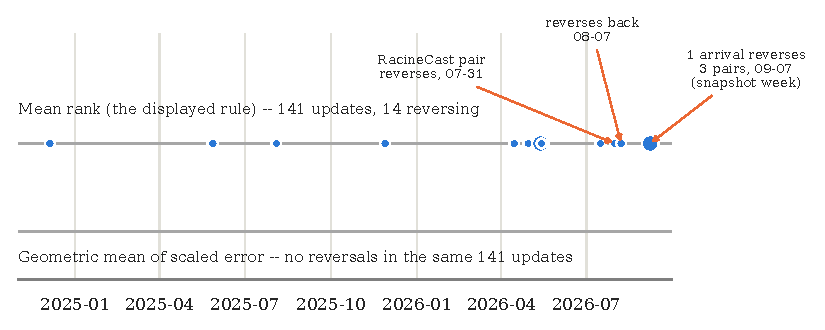
\includegraphics[width=\linewidth]{fig_timeline.pdf}
\caption{GIFT-Eval updates from 2024-11 to 2026-09 that reversed untouched top-ten pairs,
under mean rank on MASE in the upper lane and under the geometric mean of scaled error in the
lower lane, with marker area growing with the number of pairs one update reversed. The figure
counts tied ranks as averaged, which gives 18 pairs in 14 of the 141 updates, while the
board's exact tie-break gives 20 pairs (Table~\ref{tab:replay}).}
\label{fig:timeline}
\end{figure}

\paragraph{Perturbing the pool.}\label{app:perturb} The snapshot holds 131 entries with result files, and 121 of
them lie outside the top ten (three of them not displayed). Removing any one of these 121
reorders the top ten in 28 cases. Adding a near-copy of one displayed entry, for each of the
128 displayed entries including the top ten, reorders the top ten in 42 cases. The three
entries with result files that are not displayed are GestaltCog/Zeus-100M, Zeus and
iTransformer. The three newest entries of the top ten, RegLab-AH-1, TIMEHEDGE and LS-MoE, all
arrived on 2026-09-07. Dropping them reorders the seven entries that remain
(Table~\ref{tab:perturb}). The order of Falcon-Agent, CastStar and limix\_moe reverses
completely, while the other four keep their places. Only the arrival of LS-MoE reverses these
three pairs, in rows 18 to 20 of Table~\ref{tab:replay}, and none of the three entries was
rerun.

\begin{table}[htbp]
\centering
\small
\begin{tabular}{@{}lrrrr@{}}
\toprule
& \multicolumn{2}{c}{Without the three newest} & \multicolumn{2}{c}{With them} \\
\cmidrule(lr){2-3}\cmidrule(lr){4-5}
Entry & Place & Mean rank & Place & Mean rank \\
\midrule
limix\_moe & 4 & 20.59 & 7 & 22.24 \\
CastStar & 5 & 20.76 & 6 & 22.23 \\
Falcon-Agent & 6 & 20.85 & 5 & 22.15 \\
\bottomrule
\end{tabular}
\caption{Places and mean ranks on MASE of three entries of the displayed top ten, without and
with RegLab-AH-1, TIMEHEDGE and LS-MoE in the pool. A lower mean rank is better. None of the
three entries shown was rerun.}
\label{tab:perturb}
\end{table}

\paragraph{Updates since the snapshot.} Between 2026-09-07 and a second snapshot on 2026-11-13,
GIFT-Eval took 38 more updates. They reversed 8 more untouched top-ten pairs, in 8 of the 38
updates, identically under both tie conventions. Seven of the eight are limix\_moe and
EXAONE-Forecast-Agent exchanging places as other entries arrived. This happened on 2026-10-16,
2026-10-17, twice on 2026-10-23, on 2026-10-29 and twice on 2026-10-30. For example, before
HART-36M arrived on 2026-10-29 the mean ranks were 26.938 for limix\_moe and 26.949 for
EXAONE-Forecast-Agent. Afterwards they were 27.144 and 27.103. The eighth reversal is
PERSONA-AI-T4 and Timestral-209M on 2026-10-23. The whole history now holds 179 updates, with
26 reversed pairs when tied ranks are averaged and 28 under the exact tie-break.


\section{Other boards}
\label{app:boards}

\paragraph{Which boards.} We analysed every forecasting board whose per-entry, per-unit scores
could be obtained. Besides GIFT-Eval, these are fev-bench \citep{fevbench} and its smaller
version fev-bench-mini. They also include Chronos Benchmark II \citep{chronos}, BOOM
\citep{boom} and TIME \citep{timebench}. fev-bench shows 40 entries on 100 tasks from 39 task families and sorts by
win rate. fev-bench-mini scores 40 entries on 20 tasks from 15 families. Chronos Benchmark II
scores 21 entries on 27 tasks from 19 sources and fixes no rule. Of the three rules it reports,
win rate and mean rank give the same order by arithmetic, so we list mean rank and the
geometric mean. BOOM ranks 23 entries on 6,750 rows, one per series and horizon, drawn from
2,554 series of one company's monitoring data. It sorts by mean rank on its probabilistic loss.
TIME scores 43 entries on 98 units from 39 datasets and sorts by the geometric mean of scaled
MASE. The units of each board, and what counts as an independent source on it, were fixed
before any of its scores was analysed.

Chronos Benchmark I, OpenTS/TFB, ProbTS, FoundTS, Time-Series-Library and the Monash archive
repository publish no per-entry, per-unit file, so we could not analyse them. OpenTS/TFB keeps
its scores behind a private interface, ProbTS publishes formatted tables only, and the
repository of FoundTS no longer exists. TSFM-Bench publishes code without result files.
TS-Arena publishes per-entry scores, but it sorts by a rating whose update formula is not
published. Its displayed order therefore cannot be reproduced, which we required of every
board, and we did not run the report on it. LiveHouse-TS and Impermanent could not be found.
No board was dropped because of its results.

\paragraph{Reproduction.} Every analysis first had to reproduce the board's own numbers. On
fev-bench, fev-bench-mini and Chronos Benchmark II our scores match the board's own leaderboard
function exactly. BOOM publishes three decimals. Our values match its table in all six columns
at that precision, and in order for all 23 entries. BOOM breaks tied ranks by the order in
which its result files are listed. Another order moves mean ranks by up to 0.09 without
changing the displayed order. On TIME our scores match the board's own function for all 43
entries.

\begin{table}[h]
\centering
\scriptsize
\setlength{\tabcolsep}{3pt}
\begin{tabular}{@{}p{3.6cm}rrrrcp{2.9cm}@{}}
\toprule
\textbf{Board and rule} & \textbf{Sources} & \textbf{Resolution} & \textbf{Median gap} &
\textbf{Ratio} & \textbf{Neighbours separated} & \textbf{Untouched top-ten pairs reversed} \\
\midrule
GIFT-Eval, mean rank on MASE$^\dagger$ & 28 & 6.80 & 0.91 & 7.5 & 0 / 1 / 1 & 20 in 14 of 141 updates \\
GIFT-Eval, geometric mean & 28 & 0.0497 & 0.0045 & 11 & 2 / 0 / 0 & 0 in 141 \\
fev-bench, win rate$^\dagger$ & 39 & 7.51 & 2.08 & 3.6 & 0 / 0 / 0 & 2 in 2 of 30 \\
fev-bench, skill score & 39 & 3.20 & 0.83 & 3.9 & 0 / 0 / 0 & 0 in 30 \\
fev-bench-mini, win rate$^\dagger$ & 15 & 15.3 & 2.18 & 7.0 & 1 / 1 / 1 & not replayed \\
Chronos Benchmark II, mean rank$^\dagger$ & 19 & 4.24 & 0.22 & 19 & 1 / 0 / 0 & 8 in 3 of 11 \\
Chronos Benchmark II, geometric mean & 19 & 9.29 & 0.59 & 16 & 0 / 0 / 0 & 0 in 11 \\
TIME, geometric mean (displayed) & 39 & 0.0238 & 0.0021 & 11 & 1 / 0 / 1 & 0 in 44 \\
TIME, MASE rank column$^\dagger$ & 39 & 4.01 & 0.378 & 11 & 1 / 1 / 1 & 13 in 12 of 44 \\
BOOM, each series independent$^\dagger$ & 2,554 & 0.196 & 0.312 & 0.63 & 9 / 9 / 9 & history too short \\
BOOM, domain-and-type groups$^\dagger$ & 36 & 0.420 & 0.312 & 1.35 & 7 / 6 / 6 & --- \\
BOOM, domain groups$^\dagger$ & 23 & 0.635 & 0.312 & 2.04 & 7 / 5 / 6 & --- \\
\bottomrule
\end{tabular}
\caption{The report on every board. Resolution is under CR2, and the ratio is the resolution
divided by the median gap between displayed neighbours. Neighbours separated are out of 9,
uncorrected, under the submitted version's rule, CR2 and the wild cluster bootstrap. A dagger
marks rules that rank an entry against the other entries. Resolution and gap are in rank places
for mean ranks, win-rate points for win rate and rank points for BOOM. For the geometric means
of GIFT-Eval and TIME they are log ratios, and for fev-bench's skill score and Chronos Benchmark
II's geometric mean log ratios times 100. Pins: GIFT-Eval 2026-09-07, TIME 2026-10-31, the
other boards 2026-11-11. GIFT-Eval's 20 reversals use the board's exact tie-break, and with
tied ranks averaged the count is 18. TIME's counts come from the full replay of its 44
updates.}
\label{tab:boards}
\end{table}

\paragraph{The report on every board.} Table~\ref{tab:boards} gives the report on all five
boards. Every board built from 15 to 39 independent public data sources displays neighbours 3 to 20 times
closer together than it can detect. Each of them separates at most one of nine neighbouring
pairs under CR2 and the wild cluster bootstrap. This holds under mean rank, win rate, skill
score and geometric mean alike. With 20 tasks, fev-bench-mini has twice the resolution of the
full board, 15.3 against 7.5 win-rate points, at about the same median gap.

BOOM is the exception. With each of its 2,554 series counted as independent evidence, its
resolution of 0.196 rank points is finer than the median gap of 0.312. All nine neighbouring
pairs then separate under every method, which shows that the report can find a board's order
resolved. That result rests on treating series from one company's monitoring data as independent.
Grouped by domain into 23 groups, five neighbouring pairs separate under CR2. One domain holds
44\% of the rows, which leaves CR2 with about 1.6 degrees of freedom.

\paragraph{BOOM after the Holm correction.} Over all 45 top-ten pairs, CR2 separates 9 after
the Holm correction with the 23 domain groups and 36 with the 36 domain-and-type groups. The
wild cluster bootstrap and the two exact sign-flip tests separate 38 or 39 pairs with 23 groups
and 40 with 36 groups. Neither method's error rate was checked on groups this uneven, because
our simulations used the layouts of GIFT-Eval and fev-bench. We therefore quote both counts and
do not choose between them.

\paragraph{fev-bench's history.} The submitted version could not replay fev-bench. It reported
instead that removing any single entry from the September table reverses no top-ten pair. The
board's repository now holds 32 commits of results. We replayed its 30 updates under win rate
with the board's own function, and 2 of them reversed an untouched top-ten pair. The first came
on 2026-10-14 with the arrival of timeh2o-v1-tiny. ChakraTS fell from 85.39 to 84.66 and
TimesFM-3 from 85.26 to 84.91, so the two exchanged second and third place. The second came on
2026-10-15 with the arrival of TimeRSI. TiRex-2 fell from 73.22 to 71.58 and Toto-2.0-2.5B
from 73.06 to 71.67, so the two exchanged eighth and ninth place. Under the skill score no
update reversed a pair.

On the current board of 40 entries, removing one entry from outside the top ten reorders the
top ten in 2 of 30 cases. Adding a near-copy of one entry reorders it in 8 of 40 cases. The
current board separates 0 of 9 neighbours, where the September table separated 1. fev-bench
therefore shows the same effect as GIFT-Eval at a lower rate, with 2 reversed pairs in 30
updates against 20 in 141.

\paragraph{TIME's full history.} The first round scored only 29 of TIME's 45 states, because
its loader kept only files identical to the current ones. The earlier files and the earlier
baseline are all in the board's repository history. We scored every state up to 2026-10-31
with the files and the baseline as they were, on every entry present. The recomputed order
equals the board's displayed order in 45 of 45 states. Table~\ref{tab:timehist} gives the
counts. A data refresh on 2026-06-02 changed the baseline and 13 of 22 entries. We count that
update apart, and it reversed no pair. Three events in the rank columns involve two entries
that were identical on 96 of 98 units for three minutes. With the opposite tie order the
counts move by at most one. One event follows the removal of a duplicate entry rather than an
arrival. We rebuilt every past state with today's board code, and the four entries added on
2026-11-11 are not in the replay.

\begin{table}[h]
\centering
\small
\begin{tabular}{@{}lrrrl@{}}
\toprule
\textbf{Rule} & \textbf{Updates} & \textbf{With a reversal} & \textbf{Pairs} & \textbf{First round} \\
\midrule
Geometric mean of scaled MASE (displayed) & 44 & 0 & 0 & 0 in 28 \\
Geometric mean of scaled CRPS & 44 & 0 & 0 & 0 in 28 \\
MASE rank column & 44 & 12 & 13 & 6 pairs in 5 of 28 \\
CRPS rank column & 44 & 5 & 6 & 4 pairs in 4 of 28 \\
\bottomrule
\end{tabular}
\caption{Untouched top-ten pairs reversed on TIME, replayed over its whole history on the pool
the board showed. The last column gives the first round's count on a smaller pool and fewer
updates.}
\label{tab:timehist}
\end{table}

\paragraph{Chronos Benchmark II with flagged results.} On this board 74 results are flagged as
trained on the test dataset. They belong to three Moirai sizes on 22 tasks each and two TimesFM
versions on 4 tasks each. Only 5 of the 27 tasks carry no flag. The board's software
ignores the flag unless the caller names a model whose result replaces the flagged one. The
first round kept the flagged results, which is the software's default. With the flagged results
replaced by Chronos-Bolt's, mean rank has a resolution of 4.53 and a ratio of 12. It separates
1 of 9 neighbours under each of the three methods, and its history shows 4 reversed pairs in 2
of 11 updates. The geometric mean then has a ratio of 23, separates no neighbour, and reverses
no pair. With the flagged tasks dropped, 5 tasks from 4 sources remain, which is too few to say
anything. The choice of Chronos-Bolt as the replacement was ours, made after reading the
board's software.

\begin{table}[h]
\centering
\scriptsize
\setlength{\tabcolsep}{4pt}
\begin{tabular}{@{}lrrrrrcl@{}}
\toprule
\textbf{Group} & \textbf{Configurations} & \textbf{Sources} & \textbf{Resolution} &
\textbf{Median gap} & \textbf{Ratio} & \textbf{Neighbours separated} & \textbf{Leader} \\
\midrule
Full board & 97 & 28 & 6.80 & 0.91 & 7.5 & 0 / 1 / 1 & STRIDE w/ Synapse \\
Short horizon & 55 & 28 & 8.38 & 1.22 & 6.9 & 0 / 0 / 0 & STRIDE w/ Synapse \\
Medium horizon & 21 & 14 & 11.0 & 1.24 & 8.9 & 0 / 0 / 0 & STRIDE w/ Synapse \\
Long horizon & 21 & 14 & 13.4 & 0.67 & 20 & 0 / 0 / 0 & STRIDE w/ Synapse \\
Univariate & 54 & 20 & 11.8 & 0.65 & 18 & 0 / 0 / 0 & STRIDE w/ Synapse \\
Multivariate & 43 & 8 & 7.95 & 0.21 & 38 & 0 / 0 / 0 & STRIDE w/ Synapse \\
Hourly & 31 & 13 & 14.7 & 1.45 & 10 & 0 / 0 / 0 & STRIDE w/ Synapse \\
Minutely & 30 & 10 & 10.7 & 0.40 & 27 & 0 / 0 / 0 & STRIDE w/ Synapse \\
Daily & 15 & 15 & 17.0 & 1.67 & 10 & 0 / 0 / 0 & EXAONE-Forecast-Agent \\
Weekly & 8 & 8 & 36.7 & 1.63 & 23 & 0 / 0 / 0 & LS-MoE \\
Econ/Fin domain & 6 & 6 & 21.3 & 0.50 & 43 & 0 / 0 / 0 & CastStar \\
\bottomrule
\end{tabular}
\caption{GIFT-Eval's sub-boards with at least 6 sources, beside the full board. Each group is
ordered by mean rank on MASE within the group, which the app does not display. Resolution is
under CR2, in rank places. Neighbours separated are out of 9, uncorrected, under the submitted
version's rule, CR2 and the wild cluster bootstrap.}
\label{tab:subboards}
\end{table}

\paragraph{GIFT-Eval's sub-boards.} The app shows tabs by horizon, frequency, domain and variate
type. Ten of these groups have at least 6 sources, and Table~\ref{tab:subboards} reports them.
The tabs show geometric means and a mean rank on CRPS per group, with no default sort. We
therefore order each group by mean rank on MASE, to match the full board. No sub-board
separates a neighbouring pair under any method. The resolution gets coarser as the group gets
smaller. Against the number of configurations on a log scale, its slope is about $-0.5$, which
is what an inverse-square-root law predicts, with wide scatter. The leader changes in three of
the ten groups. Ten more groups have fewer than 6 sources and were not analysed. Econ/Fin, with
exactly 6, is at the edge of what any of these methods can support.

\paragraph{Variation of new datasets.} The number of datasets needed to resolve the typical gap
assumes that new datasets vary like the existing 28. Fifteen entries are scored on both
GIFT-Eval and fev-bench with the same checkpoint, 13 pretrained models and the two naive
baselines, which gives 105 pairs. For each pair we computed the spread of their log error
difference from source to source. We did this on GIFT-Eval's 28 datasets and on the 25
fev-bench families that share no data source with GIFT-Eval. The ratio of the fev-bench spread
of source means to GIFT-Eval's has a median of 1.13 over the 105 pairs, with a 95\% interval
from 0.85 to 1.72. The ratio of the per-source noise scale, which the calculation of datasets
needed uses, has a median of 1.25, with an interval from 1.11 to 1.43. On the first measure new
datasets vary about as much as the current ones, and on the second somewhat more. The
extrapolation is therefore supported but not settled, and if anything it is too small. A ratio
of 1.25 would mean about 1.5 times as many datasets again. These intervals are optimistic,
because the 15 models are closely related and horizons and window counts differ between the
boards.

\paragraph{Overlap between boards.} On fev-bench, 9 of the 39 families share a data source with
GIFT-Eval by name, and 5 more are uncertain. With all 14 removed, 67 tasks from 25 families
remain. That board separates 0 of 9 neighbours, with a resolution of 10.4 points against a
median gap of 1.4 points. On Chronos Benchmark II, 7 of 27 tasks share a source with GIFT-Eval,
and 2 more are uncertain. No TIME dataset shares a source with GIFT-Eval by name, and 8 cover
the same topic from a different provider. With those removed, TIME separates 0 of 9 under CR2,
at a ratio of 16. BOOM's data come from Datadog's internal monitoring, and no public dataset is
named. The entries overlap far more than the data. Of BOOM's 23 models, 15 match GIFT-Eval
entries by name and 5 more match with the version unconfirmed. At least 15 of fev-bench's
entries are also on GIFT-Eval.

\paragraph{The boards at a later pin.} We read GIFT-Eval again on 2026-11-13, and its updates since the snapshot are in Appendix~\ref{app:replay}.
At the new pin the board displays 170 entries. Its resolution under CR2 is 17.28 rank
places against a median gap of 0.48, and no neighbouring pair separates under any of the three
methods. Rank places stretch as entries are added, so part of the rise from 6.8 is a change of
scale. The ratio of resolution to median gap rose from 7.5 to about 36. TIME on 2026-11-11
displays 47 entries. Its resolution is 0.0235 against a median gap of 0.0021, and its
neighbour counts are unchanged.

Timestral-209M is on all three boards under that name. It is 11th on GIFT-Eval, 3rd on TIME and
4th on fev-bench. It is not separated from either neighbour on any board. Its smallest p-value
against a neighbour is 0.11, against the entry above it on fev-bench under the submitted
version's rule. TimesFM-3 is 28th on GIFT-Eval, 13th on TIME and 9th on fev-bench. The exact
tests and the known-difference control were not run at the new pin.


\section{The history-length experiment}
\label{app:history}

\paragraph{Eligible configurations.} A configuration is eligible when the median series of its
underlying data holds at least 1,024 steps. A series shorter than 512 steps shows a model the
same truncated history under both settings, and 1,024 is about twice 512. Of GIFT-Eval's 97
configurations, 70 are eligible, and all 27 that are not have a short horizon. The 70 come from
18 base datasets, which we group into 14 sources. The three bizitobs datasets form one source,
the two ETT datasets another and the two bitbrains datasets a third, because each group shares
data. Every other base dataset is its own source.

\paragraph{The first round's twelve.} The submitted version ran 12 of the 70, chosen by a rule
fixed before any model ran. The rule splits 12 slots across the three horizons in proportion
to their eligible counts, by the largest-remainder method. This gives 5 short, 3 medium and 4
long. Each horizon is then filled by shuffling its eligible configurations under a fixed seed
and picking greedily. The one hard rule is that all 12 come from distinct base datasets. Two
soft preferences follow it, taking a new domain and a new sampling frequency first, then a new
frequency only, then anything left. The 12 come from 9 sources. Version 1 of the rule had no
length filter. A review before any run found that three of its twelve picks had median series
lengths of 35, 52 and 220 steps. Those three could not have shown an effect of history
length. Both versions ship in the release. The present round ran all 70 eligible
configurations.

\paragraph{Models and documented history lengths.} The four models are Chronos-Bolt-base,
Moirai-2.0-R-small, TimesFM-2.5-200M and Toto-Open-Base-1.0, run for inference only. The
documented history length is the value in GIFT-Eval's reference notebook for each model. It is
2,048 steps for Chronos-Bolt and 4,000 for Moirai-2.0. For TimesFM-2.5 the notebook passes the
series' full history up to 15,360 steps, so 15,360 is a cap rather than the history every
series received. Toto receives the smaller of 4,096 and the longest history available, which is
4,096 on 59 of the 70 configurations. The other setting gives every model the last 512 steps.
Moirai-2.0's checkpoint reports a maximum length of 512 while its notebook passes 4,000. On the
first round's 12 configurations its two settings gave different forecasts, with a median
difference of 3.7\% and a maximum of 29.8\%. Chronos-Bolt's entry on the board declares
test-data leakage. We kept it because the design named it before any run.

\paragraph{Check of the new machine.} Chronos-Bolt, Moirai-2.0 and TimesFM-2.5 were run again
at both lengths on the first round's 12 configurations. All 72 values matched the first round,
with a largest relative difference of $2.08\times10^{-5}$ against a pass mark of $10^{-4}$. No
configuration's change between the two lengths changed sign.

\paragraph{Effect and tests.} The effect of a model is how much higher its error is with the
last 512 steps than with its documented history length. For each configuration we take the log
of MASE at 512 steps divided by MASE at the documented length. The mean over configurations,
turned back into a percentage, is the effect. It equals the change in the geometric mean of
scaled MASE. The first test asks whether the effect differs from zero. It is an exact sign-flip
test on the 14 source totals, which lists all $2^{14}$ sign patterns. It is two-sided, at 5\%,
with the Holm correction over the four models, and the 95\% interval inverts it. The second
test asks whether the effect is larger than the spread of the displayed top ten on the same
configurations. That spread is the largest of the ten entries' geometric means of scaled MASE
divided by the smallest, minus one. It is 11.76\% on the 70, 12.71\% on the 58 and 9.34\% on
the 12. The second test is one-sided, at 2.5\%, with the Holm correction over the four models.
A model whose first test does not reject enters it with $p = 1$. The estimate, both tests and
their order were fixed before any run. A level check measures how often the first test claims
an effect when there is none. It centres each model's per-configuration changes at zero, draws
them into the 14-source layout, and counts the draws in which the test rejects. Toto, the only
one of the four models that draws random samples, ran with seeds 42, 43 and 44, and the level
check used 20,000 simulated draws.

\begin{table}[h]
\centering
\scriptsize
\setlength{\tabcolsep}{4pt}
\begin{tabular}{@{}lrlllcc@{}}
\toprule
& & & & & \multicolumn{2}{c}{\textbf{False claims (\%): two-sided; rise}} \\
\cmidrule(l){6-7}
\textbf{Model} & \textbf{Effect} & \textbf{95\% interval} & \textbf{$p$} & \textbf{$p$ after Holm} &
\textbf{one value per source} & \textbf{one value per configuration} \\
\midrule
\multicolumn{7}{@{}l}{\emph{All 70 eligible configurations, 14 sources}} \\
Chronos-Bolt & +2.7\% & $-$0.9\% to +6.2\% & 0.1146 & 0.1146 & 6.01; 4.75 & 5.72; 4.26 \\
Moirai-2.0 & +6.2\% & +1.6\% to +10.4\% & 0.0051 & 0.0103 & 11.71; 0.27 & 6.26; 0.96 \\
TimesFM-2.5 & +15.3\% & +4.1\% to +32.6\% & $2.44\times10^{-4}$ & $9.77\times10^{-4}$ & 19.48; 0.07 & 7.18; 0.77 \\
Toto & +15.3\% & +4.0\% to +27.1\% & $2.44\times10^{-4}$ & $9.77\times10^{-4}$ & 13.63; 0.15 & 6.41; 0.99 \\
\addlinespace[2pt]
\multicolumn{7}{@{}l}{\emph{The 58 configurations outside the first round, 13 sources}} \\
Chronos-Bolt & +3.7\% & +0.3\% to +6.9\% & 0.0354 & 0.0354 & --- & --- \\
Moirai-2.0 & +6.1\% & +1.3\% to +11.3\% & 0.0085 & 0.0171 & --- & --- \\
TimesFM-2.5 & +14.0\% & +4.7\% to +29.3\% & $2.44\times10^{-4}$ & $9.77\times10^{-4}$ & --- & --- \\
Toto & +13.9\% & +4.4\% to +24.3\% & $2.44\times10^{-4}$ & $9.77\times10^{-4}$ & --- & --- \\
\addlinespace[2pt]
\multicolumn{7}{@{}l}{\emph{The first round's 12 configurations, 9 sources}} \\
Chronos-Bolt & $-$2.0\% & $-$8.1\% to +4.6\% & 0.9570 & 0.9570 & --- & --- \\
Moirai-2.0 & +6.8\% & +0.8\% to +12.1\% & 0.0352 & 0.1055 & --- & --- \\
TimesFM-2.5 & +22.2\% & $-$0.1\% to +55.9\% & 0.0547 & 0.1094 & --- & --- \\
Toto & +22.0\% & +1.8\% to +45.2\% & 0.0156 & 0.0625 & --- & --- \\
\bottomrule
\end{tabular}
\caption{Effect of cutting the history to 512 steps, with the exact sign-flip test on source
totals. Each set of configurations has its own Holm correction over the four models. The
columns on false claims give the level check, run on the 70 only, as the rate of false claims
of an effect in either direction and of a rise. Toto's rows use the reference notebook's setting and the
first seed.}
\label{tab:g1}
\end{table}

\paragraph{Effect on the 70 configurations.} On the 70 configurations the first test rejects
after the Holm correction for three models (Table~\ref{tab:g1}). Moirai-2.0's error rises by
6.2\%, with a 95\% interval from +1.6\% to +10.4\%. TimesFM-2.5's error rises by 15.3\%, with
an interval from +4.1\% to +32.6\%. Toto's error also rises by 15.3\%, with an interval from
+4.0\% to +27.1\%. No effect is established for Chronos-Bolt, at +2.7\% with $p = 0.1146$.

For the three models the test also rejects on the 58 configurations outside the first round.
The effect is therefore confirmed on configurations that did not suggest it. These 58 are not
fully separate from the first round. Of them, 43 come from a base dataset already among the 12,
and 20 use the same series as one of the 12 at another horizon. Chronos-Bolt also rejects on
the 58, at +3.7\% with $p = 0.0354$ after Holm. However, the 70 are the test of record, and
its change of $-2.0\%$ on the 12 does not recur on the 58. The level check below also shows
that the test claims a rise too often for this model, so we make no claim for it. On the first
round's 12 configurations alone, with sources as groups, no model's effect survives the Holm
correction. The smallest corrected p-value there is Toto's 0.0625.

\paragraph{Rates of false claims.} On changes this skewed the two-sided test does not hold its
5\% level. In the level check it claims an effect in 6.01\%, 11.71\%, 19.48\% and 13.63\% of
draws for Chronos-Bolt, Moirai-2.0, TimesFM-2.5 and Toto. One direction of a two-sided 5\%
test should claim in 2.5\%. For Moirai-2.0, TimesFM-2.5 and Toto, whose changes have a long
tail on the side of a rise, a false claim of a rise occurs in at most 1\% of simulated draws.
With the tail on the other side the same test would claim a rise in 12\% to 19\% of draws.
With one value drawn per configuration, the rates of a false rise are 0.96\%, 0.77\% and
0.99\%. With one value per source they are 0.27\%, 0.07\% and 0.15\%. The skewness of the
three models' changes is +2.41, +2.80 and +2.23, and about 70\% of their configurations lie
below the mean. The rate of at most 1\% therefore holds for changes of this shape.

TimesFM-2.5 and Toto also pass a plain count that needs no assumption about shape. For each of
them the error rises on 64 of the 70 configurations and in 13 of the 14 sources. The
fourteenth source, m4\_daily, is at zero by rule for Toto and at $-0.3\%$ for TimesFM-2.5.
Moirai-2.0's error rises in 10 of the 14 sources and on 51 of the 70 configurations. Its result
therefore rests on the size of the rises as well as on their number. Chronos-Bolt's changes
are skewed the other way, with a skewness of $-1.53$. A false claim of a rise occurs for it in
4.75\% of draws, above the 2.5\% one direction should have. We make no claim for Chronos-Bolt,
but its p-values on the 58 and the 70 should not be read as conservative.

\paragraph{Leaving one source out.} Leaving one source out of the 70 moves the effect of
TimesFM-2.5 between +6.7\% and +17.7\%, and that of Toto between +9.3\% and +16.7\%. For
Moirai-2.0 the range is +4.1\% to +6.9\%, and for Chronos-Bolt +1.9\% to +4.1\%. For the three
models with an effect, the lowest value comes from leaving out the bizitobs source.

\paragraph{The test against the spread.} The second test rejects for no model, on the 70, the
58 or the 12. On the 70 its p-value after Holm is 1.0000 for every model. The intervals of
TimesFM-2.5 and Toto reach down to about 4\%, below the spread of 11.76\%. The data therefore
do not establish that any model's effect is larger than the spread of the displayed top ten.
This test has limits. Firstly, it uses the spread as a fixed yardstick, although the spread
is itself computed from data. Leaving one base dataset out of the 70 moves it between 8.51\%
and 13.22\%. Secondly, 14 sources is few. The smallest two-sided p-value possible is
$2/2^{14}$, and a single large source can still carry a sum.

\begin{table}[h]
\centering
\scriptsize
\setlength{\tabcolsep}{4pt}
\begin{tabular}{@{}lrrlllccl@{}}
\toprule
& & & & & & \multicolumn{2}{c}{\textbf{False claims (\%): two-sided; rise}} & \\
\cmidrule(lr){7-8}
\textbf{Model} & \textbf{Board} & \textbf{Effect} & \textbf{95\% interval} & \textbf{$p$} &
\textbf{$p$ after Holm} & \textbf{per source} & \textbf{per configuration} &
\textbf{Spread test} \\
\midrule
TimesFM-3 & 0.6750 & +31.8\% & +5.3\% to +69.4\% & 0.0156 & 0.0156 & 16.32; 0.10 & 13.39; 0.19 & 0.1094 \\
Timestral-209M & 0.6521 & +28.9\% & +6.3\% to +54.1\% & 0.0039 & 0.0078 & 10.12; 0.38 & 8.20; 0.56 & 0.1094 \\
\bottomrule
\end{tabular}
\caption{Two newer models on the first round's 12 configurations, from 9 sources, with the Holm
correction over the two models. The board column gives the geometric mean of scaled MASE of
the board's published rows, which our runs reproduce at the documented history length. The
last column is the p-value after Holm of the test against the spread of the displayed top ten,
which is 9.34\% on the 12. Twelve configurations from nine sources give wide intervals.}
\label{tab:g2}
\end{table}

\paragraph{Two newer models.} TimesFM-3 \citep{timesfm} and Timestral-209M \citep{timestral}
ran on the first round's 12 configurations with the same tests. The Holm correction runs over
the two models, and the level check uses the layout of 9 sources. Both reproduce the board's published rows at the
documented history length, with a largest relative difference of $1.5\times10^{-7}$.
Timestral-209M's rows come from the board as read on 2026-11-13, because the model is not in
the September snapshot. Seasonal Naive's values and the spread on the 12 are the same at both
pins. TimesFM-3's error rises by 31.8\% at 512 steps, with an interval from +5.3\% to +69.4\%
and $p = 0.0156$ after Holm. Timestral-209M's rises by 28.9\%, with an interval from +6.3\% to
+54.1\% and $p = 0.0078$ after Holm (Table~\ref{tab:g2}). The test against the spread rejects
for neither. Twelve configurations from nine sources give these wide intervals. The larger rate
of a false rise is 0.19\% for TimesFM-3 and 0.56\% for Timestral-209M, and as above it holds
for changes with their long tail on the side of a rise. TimesFM-3 receives the full history up
to 15,360 steps. Timestral-209M receives the most recent 32,768 steps at most, and 5 of the 12
configurations reach that limit.

\begin{table}[h]
\centering
\small
\begin{tabular}{@{}lrrrr@{}}
\toprule
\textbf{Toto run} & \textbf{Documented length} & \textbf{Against the board} & \textbf{512 steps} & \textbf{Effect} \\
\midrule
First round, one point forecast & 0.8126 & +5.54\% & 0.9801 & +20.6\% \\
Notebook's setting, first seed & 0.7698 & $-$0.02\% & 0.9391 & +22.0\% \\
Notebook's setting, second seed & 0.7692 & --- & 0.9388 & +22.1\% \\
Notebook's setting, third seed & 0.7709 & --- & 0.9380 & +21.7\% \\
\bottomrule
\end{tabular}
\caption{Toto on the first round's 12 configurations, as the geometric mean of scaled MASE.
The board's published rows give 0.7699. The reference notebook's setting draws 256 samples and
scores their median. The first seed is the value of record.}
\label{tab:toto}
\end{table}

\paragraph{Toto's reproduction.} In the submitted version our Toto run scored 0.8126 on the 12
configurations, against 0.7699 from the board's published rows. The first round passed no
sample count, so the model returned one point forecast. The present round used the reference
notebook's setting. It draws 256 samples and scores their median, and it keeps the key-value
cache on. It also sets two numeric switches, one for faster matrix products and one for
deterministic algorithms. With the reference notebook's setting our run reproduces the board's published rows
(a difference of 0.02\% on the twelve configurations and 0.01\% on the 70). The submitted
version's run differed mainly in scoring one point forecast instead of the median of 256
samples. We attribute its 0.813 to this, because the other differences should not move the
expected score. We did not rerun the earlier setting to isolate it.

With one point forecast, single configurations were off by up to 28.55\%. With the notebook's
setting none of the 12 configurations is off by more than 0.28\%, and none of the 70 by more
than 0.49\%. The board's value lies inside the range of the three seeds, 0.7692 to 0.7709
(Table~\ref{tab:toto}). Over the three seeds the effect runs from +21.7\% to +22.1\%, a range of
0.38 percentage points. In 8 of Toto's 185 runs the card ran out of memory with all 256
samples drawn at once. Those runs drew the samples in batches of 64 or 32, as the board's
notebook does, and each forecast still uses 256 samples.

\paragraph{What the Toto run does not separate.} The notebook's setting changes the sample
count, the key-value cache, the two numeric switches and the batch size together. The run
therefore does not show which part alone closes the gap. The first round's setting was not run
again on the new machine, so its 0.8126 is the first round's value. The first round's run
record leaves Toto's model revision blank. Before the runs we checked that the published
revision had not changed since September. The variant without the faster matrix products was
not run, because the reproduction check passed.


\section{Additional tables and selection details}
\label{app:tables}

\subsection{What did the submitted version's twelve-configuration runs show?}
\label{app:gridfull}

This subsection reports the submitted version's runs on twelve configurations. Toto's rows
in it come from a run that scored one point forecast, and the runs of record are in
Appendix~\ref{app:history}.

\begin{table}[h]
\centering
\scriptsize
\setlength{\tabcolsep}{3pt}
\begin{tabular}{lrlrrrl}
\toprule
 & \multicolumn{3}{c}{board's own entry} & \multicolumn{3}{c}{our runs} \\
\cmidrule(lr){2-4}\cmidrule(lr){5-7}
Model & score & \multicolumn{1}{c}{95\% band} & half-width & default & 512 & \multicolumn{1}{c}{$\Delta$ (95\% CI)} \\
\midrule
\multicolumn{7}{l}{\emph{Mean insertion rank}} \\
Chronos-Bolt-base\,$^\dagger$ & 79.58 & [61.92, 97.58] & 17.83 & 80.33 & 87.00 & +6.67 [$-$4.92, +19.00] \\
Moirai-2.0-R-small & 62.83 & [43.75, 80.17] & 18.21 & 63.33 & 67.42 & +4.08 [$-$6.92, +14.08] \\
TimesFM-2.5-200M & 61.75 & [49.58, 73.33] & 11.87 & 62.25 & 88.83 & \textbf{+26.58 [+8.83, +44.42]} \\
Toto-Open-Base-1.0 & 69.08 & [57.42, 81.08] & 11.83 & 82.08 & 98.67 & \textbf{+16.58 [+6.50, +28.00]} \\
\midrule
\multicolumn{7}{l}{\emph{Geometric mean of scaled MASE}} \\
Chronos-Bolt-base\,$^\dagger$ & 0.9676 & [0.7081, 1.3673] & 0.3296 & 0.9650 & 0.9461 & $-$0.0189 [$-$0.175, +0.063] \\
Moirai-2.0-R-small & 0.7233 & [0.6258, 0.8303] & 0.1023 & 0.7233 & 0.7727 & \textbf{+0.0494 [+0.006, +0.107]} \\
TimesFM-2.5-200M & 0.7348 & [0.6293, 0.8428] & 0.1068 & 0.7348 & 0.8977 & \textbf{+0.1629 [+0.040, +0.342]} \\
Toto-Open-Base-1.0 & 0.7699 & [0.6938, 0.8488] & 0.0775 & 0.8126 & 0.9801 & \textbf{+0.1675 [+0.067, +0.317]} \\
\bottomrule
\end{tabular}
\caption{The submitted version's runs on the 12 configurations, kept as a record and superseded by Table~\ref{tab:g1}. Mean insertion rank is the mean rank on MASE of a run entered into the board's pool as an extra entry. The board columns hold each entry's published score and the 95\% band from resampling configurations, with no runs of ours. Default is the documented history length. A positive $\Delta$ is worse. Bold marked a percentile-bootstrap interval excluding zero, a rule this version withdraws (Appendix~\ref{app:changes}). Toto's default column is the run that scored one point forecast. The dagger marks the leakage-flagged entry.}
\label{tab:grid}
\end{table}



\subsection{How much history did the models actually receive?}
\label{app:ctx}

A documented history length binds only where the series is long enough to supply it, and many
series here are not. A board requesting this field should request the history received
rather than the argument passed.

\begin{table}[h]
\centering
\small
\setlength{\tabcolsep}{6pt}
\begin{tabular}{llrr}
\toprule
Model & configuration & documented & received \\
\midrule
Chronos-Bolt-base & us\_births/W/short & 2048 & 983 \\
Moirai-2.0-R-small & us\_births/W/short & 4000 & 983 \\
TimesFM-2.5 & us\_births/W/short & 15{,}360 & 983 \\
Toto & bizitobs\_l2c/H/long & 4096 & 1224 \\
Toto & m4\_daily/D/short & 4096 & 79 \\
\bottomrule
\end{tabular}
\caption{Five of the 13 cells where the documented history length did not bind, measured at the median evaluation
window. Three models with documented contexts of 2048, 4000 and 15{,}360 steps received the same
983 (Figure~\ref{fig:received}).}
\label{tab:effctx}
\end{table}

Counted by the median evaluation window, 13 of the 48 default-setting cells received less history
than documented, with 14 by the minimum window and 12 by the maximum, and the release ships the
effective context per cell. Toto's m4\_daily cell receives
79 steps under both settings, so that cell measures nothing.
The documented default history lengths are 2048, 4000, 15360 and 4096 steps for Chronos-Bolt-base,
Moirai-2.0-R-small, TimesFM-2.5 and Toto in that order, all four capped by available history.
Datadog's benchmark chose 2048 after preliminary experiments showed 512 degrading performance
across models \citep{boom}.

\begin{figure}[h]
\centering
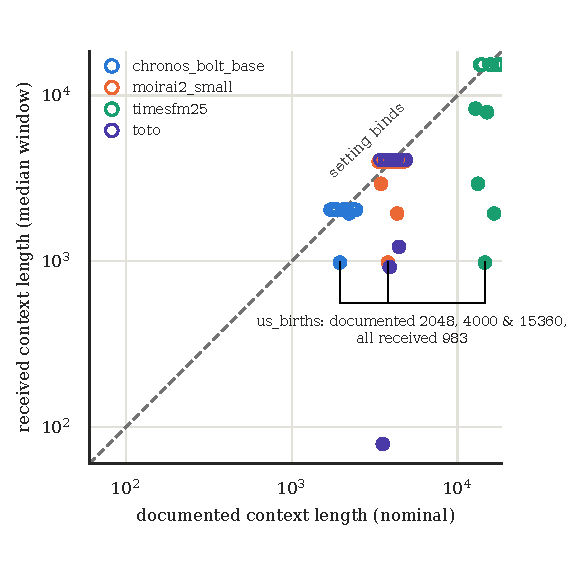
\includegraphics[width=0.7\linewidth]{fig_received.pdf}
\caption{Documented vs.\ received history length: the 48 default-setting runs,
plotting each run's documented (nominal) history length against the history
length it actually received, measured at the median evaluation window. The
dashed diagonal is $y=x$, where the documented setting binds; open circles sit
on it, filled circles sit below it. The bracketed points are \texttt{us\_births}:
Chronos-Bolt-base, Moirai-2.0-R-small and TimesFM-2.5 document 2048, 4000 and
15{,}360 steps of context respectively, but all received 983 at the median window. 13 of the 48
default-setting runs received less history than documented, counted at the
median window.}
\label{fig:received}
\end{figure}


\section{Declared fields}
\label{app:census}

\begin{table}[h]
\centering
\small
\begin{tabular}{@{}lrr@{}}
\toprule
\textbf{Declared field} & \textbf{All 130 registered entries} & \textbf{Displayed top ten} \\
\midrule
No reproduction code & 55 & 9 \\
Test-data leakage & 17 & 0 \\
An agentic pipeline rather than a single model & --- & 10 \\
\bottomrule
\end{tabular}
\caption{Fields that each entry declares about itself in the pinned snapshot, which the board
does not audit. The model-type field was counted only for the displayed top ten.}
\label{tab:census}
\end{table}

The top of the board is less checkable than its average. Two entries are lost when the app
joins result files to the entries' declarations by name, and a check at ingest would catch
both. We excluded both from pairwise resampling. One model's results are labelled
\texttt{iTransformer} while its declaration names it \texttt{i\_transformer}, so an entry with
complete data never appears in the displayed table. Separately, 14 rows in the \texttt{Zeus}
results folder carry a model name that no declaration claims, which leaves Zeus with 83 of 97
configurations.


\section{Changes from the submitted version}
\label{app:changes}

Table~\ref{tab:changes} lists each statement of the submitted version that this version
changes, with what it says now and the reason.

\begin{table}[h]
\centering
\scriptsize
\setlength{\tabcolsep}{4pt}
\begin{tabular}{@{}p{4.1cm}p{4.9cm}p{4.3cm}@{}}
\toprule
\textbf{The submitted version said} & \textbf{This version says} & \textbf{Why} \\
\midrule
GIFT-Eval resolves 6.2 rank places. &
It resolves 6.8 rank places, under CR2. &
The submitted version's rule declared a difference in 6.1\% of resampled real pairs with none,
against 5.2\% for CR2 (Appendix~\ref{app:calib}). \\
\addlinespace[2pt]
No neighbouring top-ten pair separates under either rank rule. &
None separates after the Holm correction, under every method. The pair at places 9 and 10 has
$p = 0.036$ uncorrected. &
The claim holds once the correction for multiple comparisons is named. \\
\addlinespace[2pt]
Under mean rank on MASE, 12 of the 45 top-ten pairs separate, and two after a Holm correction. &
12 of 45 separate. None does after Holm under CR2, and one does under the wild cluster
bootstrap. &
CR2 replaces the percentile bootstrap. \\
\addlinespace[2pt]
Under the geometric mean, 2 of 9 neighbours and 11 pairs after Holm separate, the most of the
three rules. &
Under CR2, 0 of 9 neighbours and 10 of 45 pairs separate, and none after Holm. The usual tests
do not hold their level on this rule. &
One dataset supplies more than half the variance in 28 of 45 pairs
(Appendix~\ref{app:calib}). \\
\addlinespace[2pt]
The leading tier under the geometric mean holds nine entries, with TimesFM-3 the closest call. &
It holds 17 entries under CR2 and 16 under the signed-rank test on dataset means. TimesFM-3 is
in both. &
The corrected methods widen the tier, and the signed-rank test holds its level
(Appendix~\ref{app:tiers}). \\
\addlinespace[2pt]
About 45 times as many datasets would be needed. &
About 48 times as many, and probably more. &
CR2 gives 48, and datasets outside the board vary at least as much
(Appendix~\ref{app:boards}). \\
\addlinespace[2pt]
On fev-bench, removing any single entry reverses no top-ten pair, and fev-bench is the contrast
to GIFT-Eval. &
Two untouched top-ten pairs reversed on fev-bench in 30 updates. The contrast is the rule that
uses only an entry's own scores, which reversed no pair on any board. &
fev-bench's history became available. \\
\addlinespace[2pt]
Table~\ref{tab:report} gives fev-bench's September table. &
It gives the board as read on 2026-11-11, with 40 entries. &
The board has changed since September. \\
\addlinespace[2pt]
Cutting the history to 512 steps raises the error of TimesFM-2.5 by 22.2\% and of Toto by
20.6\%, on 12 configurations. &
On 70 configurations it raises the error of Moirai-2.0 by 6.2\%, of TimesFM-2.5 by 15.3\% and
of Toto by 15.3\%. No effect is established for Chronos-Bolt. &
We ran all 70 eligible configurations. \\
\addlinespace[2pt]
Both movements survive a correction across the eight tests. &
On the 12 alone no effect survives the Holm correction with sources as groups. On the 70, three
of four do. &
An exact sign-flip test on source totals replaces the percentile bootstrap, which declared a
false difference in 8\% to 13\% of simulated cases with 12 configurations. \\
\addlinespace[2pt]
The effect is set against the 9.3\% spread of the displayed top ten, without a test. &
The test against the spread, 11.76\% on the 70, rejects for no model. &
The intervals reach down to about 4\%. \\
\addlinespace[2pt]
Toto scores 0.813 against the board's 0.770, and its effect on the 12 is +20.6\%. &
With the reference notebook's setting Toto scores 0.7698 against 0.7699, and its effect on the
12 is +22.0\%. &
The first round's run differed mainly in scoring one point forecast instead of the median of
256 samples. \\
\addlinespace[2pt]
Each model ran once per configuration and setting. &
Toto ran with three seeds, and its effect varies by 0.38 percentage points. The other three
models are deterministic. &
Only Toto draws random samples. \\
\addlinespace[2pt]
TimesFM-2.5's documented history is 15,360 steps. &
15,360 steps is a cap, and the model receives the series' full history up to it. &
This is the rule of the reference notebook. \\
\addlinespace[2pt]
A wild cluster bootstrap is the natural next check. &
It was run, with two exact sign-flip tests beside it. &
A reviewer asked for small-sample corrections. \\
\addlinespace[2pt]
GIFT-Eval and fev-bench are analysed. &
Four more boards and ten sub-boards of GIFT-Eval are analysed. &
A reviewer asked whether the findings hold beyond GIFT-Eval. \\
\addlinespace[2pt]
The checklist has four fields. &
It has five, with sampling added. &
The reference notebook's sampling setting reproduces Toto's published rows. \\
\bottomrule
\end{tabular}
\caption{What changed between the submitted version and this one. The reversal count on
GIFT-Eval, the census and the counts of received history are unchanged.}
\label{tab:changes}
\end{table}
\clearpage


\section{Validity and limitations}
\label{app:validity}

\paragraph{What the intervals answer.} They answer whether the displayed order would survive an
equally reasonable draw of datasets from this board's pool. On the fixed evaluation set the
published means are exact and carry no uncertainty of their own. The estimate of how many more
datasets would resolve the typical gap assumes that new datasets resemble the current ones.
Datasets outside the board vary somewhat more (Appendix~\ref{app:boards}), so we give the
estimate as an order of magnitude.

\paragraph{Few clusters.} GIFT-Eval has 28 clusters, and with so few the submitted version's
percentile bootstrap was too lenient (Appendix~\ref{app:calib}). CR2 and the wild cluster
bootstrap correct most of this. In simulation both stay close to 5\% except on strongly
lopsided data, where both drift to 6\% to 7\%. On fev-bench's layout, with strong correlation
within families, CR2 is too cautious at 2\% to 3\%, and the wild cluster bootstrap does better
there. CR2 stays the primary method because the rule for choosing it was fixed in advance. The
wild cluster bootstrap gives p-values only, and we computed no intervals from it.

\paragraph{Skewed changes and the sign-flip test.} The exact sign-flip test is exact only when,
with no true difference, each source total is as likely to be positive as negative. Skewed
changes break this. In the history-length experiment the two-sided test claimed an effect in
6.01\% to 19.48\% of simulated draws that had none. The rate of a false rise stayed at or below
1\% for the three models whose changes have their long tail on the side of a rise. It was
4.75\% for Chronos-Bolt, whose tail lies on the other side. The geometric mean of scaled error
on GIFT-Eval shows the same problem. There the usual tests declare a difference in about 16\%
of resampled pairs with none (Appendix~\ref{app:calib}).

\paragraph{BOOM's uneven groups.} One BOOM domain holds 44\% of the rows, which leaves CR2 with
about 1.6 degrees of freedom at 23 groups. At its own resolution there, CR2 detects a known
difference 75\% of the time and the wild cluster bootstrap 92\%, against a target of 80\%.
Both raise false alarms in 6\% of resamples. With a few dozen very unequal groups no method is
reliable, so we report both families of tests (Appendix~\ref{app:boards}). The groupings are
our reading of what series could share, since BOOM's files say nothing about correlation
between series of one domain.

\paragraph{TIME's tie events.} Three events in TIME's rank columns involve two entries that were
identical on 96 of 98 units for three minutes. The board breaks such ties by the order in which
it lists folders, which depends on the machine. With the opposite order the counts move by at
most one. Our replay rebuilt every past state with today's board code, which may differ from
the code that ran at the time.

\paragraph{The spread as a fixed yardstick.} The test against the spread of the displayed top
ten treats that spread as fixed, although it is computed from data. Leaving one base dataset
out of the 70 moves it between 8.51\% and 13.22\%.

\paragraph{What the published scores average away.} Each published score is itself a mean over
rolling windows, so our resampling captures variation between configurations and not within
them. Total uncertainty is therefore larger than what we report.

\paragraph{Sources inside the experiment.} The 70 configurations come from 18 base datasets in
14 sources. Grouping datasets that share data does not remove other dependence, such as
sources from one domain. Fourteen sources is few, and a single large source can still carry a
sum. Leaving out the bizitobs source lowers the effect of TimesFM-2.5 to +6.7\% and that of
Toto to +9.3\%.

\paragraph{Repeat runs.} Only Toto draws random samples, so only Toto was run three times. Its
effect on the 12 configurations ranged from +21.7\% to +22.1\% over the three seeds. The other
three models are deterministic. Their 72 values on the first round's configurations matched
across two machines to a relative difference of $2.08\times10^{-5}$.

\paragraph{Received history.} No log records the history each forecast window received. The 48
values behind Table~\ref{tab:effctx} and Figure~\ref{fig:received} are computed from the series
lengths and each model's rule.

\paragraph{Declared fields.} The board does not audit the declarations counted in
Table~\ref{tab:census}, and neither do we.


\end{document}
